\documentclass[
12pt, % 字体大小
a4paper, 
oneside, % 单面打印(双面为twoside)
headinclude,footinclude, % 页眉页脚包含在文本区域内,确保不被裁剪或掩盖
]{scrartcl}
% 主题和样式
\usepackage[
nochapters, % 无章节层级 
beramono, % 等宽字体样式
eulermath, % 数学公式Euler字体
pdfspacing, % 字间距
dottedtoc % 点线式目录
]{classicthesis}
\usepackage{arsclassica} 
%----------------------------------------------------------------------------------------
% 输入和页面排版
\usepackage[T1]{fontenc} % 字体编码
\usepackage[utf8]{inputenc} % 输入编码
\usepackage{ctex} % 汉语
\usepackage{amsmath,amssymb,amsthm} % 数学公式
\usepackage{indentfirst} % 缩进
\setlength{\parindent}{2em} % 段落缩进
\usepackage[
top=2cm,
bottom=2cm, 
left=2cm,
right=2cm, 
headheight=20pt, 
includeheadfoot 
]{geometry} % 页面
\usepackage{scrlayer-scrpage} % 页眉页脚
\renewcommand{\sectionmark}[1]{\markright{\spacedlowsmallcaps{#1}}}
\renewcommand{\subsectionmark}[1]{\markright{\thesubsection~#1}}
\lehead{\mbox{\llap{\small\thepage\kern1em\color{halfgray} \vline}\color{halfgray}\hspace{0.5em}\rightmark\hfil}} % 标题旁边标记页码
\cfoot{\hyperlink{toc}{\color{RoyalBlue}返回目录}} % 页脚返回目录链接
\pagestyle{scrheadings}
%----------------------------------------------------------------------------------------
% 图表和引用
\usepackage{graphicx} % 图像
\graphicspath{{Figures/}} % 图像路径
\usepackage{subfig} % 图组
\usepackage{float} % 浮动
\usepackage{enumitem} % 列表
\usepackage{varioref} % 交叉引用
%----------------------------------------------------------------------------------------
% 代码
\usepackage{listings}
\lstset{
    language=Matlab,
    basicstyle=\ttfamily\small,   % 字体
    numbers=left,                 % 行号
    numberstyle=\tiny\color{gray},
    stepnumber=5,
    numbersep=5pt,
    backgroundcolor=\color{white},% 背景
    tabsize=2,                    % 制表符宽度
    frame=single,                 % 边框
    captionpos=t,                 % 标题
    title=\lstname,
    breaklines=true,              % 换行
    breakatwhitespace=true,
    escapeinside={`}{`},          % 转义(中文注释)
}
\lstset{
    language=Python,            
    basicstyle=\ttfamily\small,   % 字体
    numbers=left,                 % 行号
    numberstyle=\tiny\color{gray}, 
    stepnumber=5,             
    numbersep=5pt,            
    backgroundcolor=\color{white},% 背景
    tabsize=4,                    % 制表符宽度            
    frame=single,                 % 边框
    captionpos=t,                 % 标题
    title=\lstname, 
    breaklines=true,              % 换行
    breakatwhitespace=false,   
    escapeinside={`}{`},          % 转义(中文注释)
}
\usepackage{algorithm} % 算法
\usepackage{algpseudocode}
\usepackage{mdframed} % 跨页框架
% 不浮动算法环境
\newcounter{myalgorithm}
\renewcommand{\themyalgorithm}{\arabic{myalgorithm}}
\newenvironment{myalgorithm}[1][]{
  \refstepcounter{myalgorithm}
  \begin{mdframed}[
    skipabove=\topskip,
    skipbelow=\topskip,
    needspace=3\baselineskip,
    linewidth=0.4pt,
    frametitlefont=\normalfont\bfseries,
    frametitle={算法 \themyalgorithm\if\relax\detokenize{#1}\relax\else:#1\fi},
    frametitlerule=true,
    frametitlerulewidth=0.4pt,
    repeatframetitle=true
  ]
  \begin{algorithmic}[1]
  \ifx\relax\detokenize{#1}\relax
    \addcontentsline{alg}{algorithms}{\makebox[7em][l]{算法~\themyalgorithm} }
  \else
    \addcontentsline{alg}{algorithms}{\makebox[7em][l]{算法~\themyalgorithm} #1}
  \fi
}{
  \end{algorithmic}
  \end{mdframed}
}
% 关键词
\algrenewcommand{\algorithmicwhile}{当}
\algrenewcommand{\algorithmicdo}{执行}
\algrenewcommand{\algorithmicend}{结束}
\algrenewcommand{\algorithmicif}{如果}
\algrenewcommand{\algorithmicthen}{那么}
\algrenewcommand{\algorithmicelse}{否则}
\algrenewcommand{\algorithmicfor}{对于}
\algrenewcommand{\algorithmicrepeat}{循环}
\algrenewcommand{\algorithmicuntil}{直到}
\algrenewcommand{\algorithmicloop}{循环}
\algnotext{EndFor}
\algnotext{EndIf}
\algnotext{EndLoop}
\algnotext{EndWhile}
%----------------------------------------------------------------------------------------
% 超链接与PDF信息
\usepackage{hyperref} 
\hypersetup{
colorlinks=true, % 彩色
breaklinks=true, % 断行
urlcolor=webbrown, % URL棕色
linkcolor=RoyalBlue, % 内部链接蓝色
citecolor=webgreen, % 引用绿色
bookmarks=true, % 书签
bookmarksnumbered,
pdftitle={}, 
pdfauthor={},
pdfsubject={}, 
pdfkeywords={}, 
pdfcreator={pdfLaTeX}, 
pdfproducer={LaTeX with hyperref and ClassicThesis} 
}
%----------------------------------------------------------------------------------------
% 目录与标题
\usepackage{titlesec} 
\AtBeginDocument{
    \renewcommand{\contentsname}{目\hspace{1em}录}
    \renewcommand{\listfigurename}{图\hspace{1em}片}
    \renewcommand{\listtablename}{表\hspace{1em}格}
    \renewcommand{\figurename}{图}
    \renewcommand{\tablename}{表}
    \setcounter{tocdepth}{3} % 目录深度
}
\theoremstyle{definition} 
\newtheorem{definition}{定义}
\theoremstyle{plain} 
\newtheorem{theorem}{定理}
\theoremstyle{remark}
\newtheorem{remark}{备注}
\newtheorem{example}{样例}
\usepackage{tocloft} % 目录
% 要点目录
\newlistof{tips}{tip}{要\hspace{1em}点}
\newcommand{\tip}[1]{
  \refstepcounter{tips}
  \textsuperscript{\textcolor{orange}{\textbf{\thetips}}}
  \addcontentsline{tip}{tips}{\makebox[7em][l]{要点~\thetips} #1}
}
% 算法目录
\newlistof{algorithms}{alg}{算\hspace{1em}法} 
\hyphenation{Fortran hy-phen-ation} % 单词断字规则
%----------------------------------------------------------------------------------------
% 题目和作者
\title{\normalfont\spacedallcaps{强化学习}} 
\date{}
%----------------------------------------------------------------------------------------
% 开始和目录
\begin{document}
\maketitle
\newpage
\hypertarget{toc}{}
\tableofcontents 
\newpage
\listoffigures
\listoftables
\listofalgorithms
\listoftips
\newpage
%----------------------------------------------------------------------------------------
\section{导论}
%------------------------------------------------
\paragraph{特征}
智能体与环境交互(采样),在不断尝试中学习策略,使收益最大化。
\begin{itemize}
\item 试错探索:不会获知应采取的行动,通过尝试获得。
\item 延迟收益:一个动作的收益可能无法短期体现,而是长期浮现。
\item 环境不确定性:当前动作不但会影响当前收益,还会影响后续环境,进而影响后续收益。
\item 影响未知性:无法预测动作的影响,需要与环境频繁交互。
\item 试探(开拓动作空间)与开发/贪心(根据经验获得收益)折中。
\end{itemize}
%------------------------------------------------
\paragraph{其他优化方法}
\begin{itemize}
\item 凸优化:状态空间较小,线性规划。
\item 最优控制:已知模型,解析回报函数,动态规划。
\item 进化算法:控制策略简单。
\item 机器学习
\begin{itemize}
\item 有监督学习:有标签,注重推断与泛化能力。
\item 无监督学习:无标签,寻找数据隐含结构。
\end{itemize}
\end{itemize}
%------------------------------------------------
\paragraph{分类}
\begin{enumerate}
\item 模型依赖性
\begin{itemize}
\item 有模型:规划。
\item 无模型:试错。
\end{itemize}
\item 策略更新方法
\begin{itemize}
\item 值函数:求解值函数重构策略。
\item 直接策略搜索:搜索策略空间。
\item Actor-Critic方法:类似于策略迭代,同时逼近值函数和策略。
\end{itemize}
\item 回报函数是否已知
\begin{itemize}
\item 正向:从回报到策略。
\item 逆向:从专家示例到回报。
\end{itemize}
\item 任务体量:分层强化学习、元强化学习、多智能体强化学习、迁移学习等
\end{enumerate}
%------------------------------------------------
\paragraph{发展}\label{sec:history back}~\\

值函数$ \rightarrow $直接策略搜索$ \rightarrow $深度强化学习。详细历史见\ref{sec:history}。

与深度学习结合,与专业知识结合,理论分析型增强,与认知科学结合,体量增大,与贝叶斯结合。
%----------------------------------------------------------------------------------------
\section{马尔可夫决策过程与贝尔曼方程}
%----------------------------------------------------------------------------------------
\subsection{马尔可夫决策过程(Markov decision process,MDP)}
%------------------------------------------------
\subsubsection{要素}\tip{马尔可夫决策过程及其元素}
\begin{itemize}
\item 状态(state,S):强化学习依赖的概念。
\item 动作(action,A):智能体做出的选择。
\item 奖励/收益(reward,R):短期学习目标,环境给予智能体的信号。
\item 策略(policy,$ \pi $):在特定状态下,动作集的分布$ \pi(a|s) = p[A_t = a|S_t = s] $。
\item 回报(return,G):长期收益累计,可能含有折扣,需综合评估。
\item 折扣因子($ \gamma $)。
\item 值函数(value function,V):一定状态下预估的期望回报。
\item 行为/动作值函数(Q):一定状态-动作对下预估的期望回报。
\item 环境模型(P):模拟环境的反应。
\end{itemize}

\begin{figure}[H]
\centering 
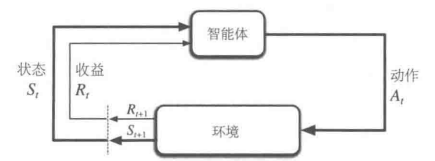
\includegraphics[width=0.5\textwidth]{Markov} 
\caption[马尔可夫决策过程]{马尔可夫决策过程}
\end{figure}
%------------------------------------------------
\subsubsection{状态、动作与收益}
%------------------------------------------------
\paragraph{序贯交互轨迹(trajectory)$ \tau =  S_0, A_0, R_1, S_1, A_1, R_2, \dots $}~\\

随机变量$ s',r $服从离散概率分布$ p(s', r|s, a) \doteq \Pr\{S_t = s', R_t = r|S_{t - 1} = s, A_{t - 1} = a\} $,即$ S_t,R_t $所有可能组合的概率和为1。
%------------------------------------------------
\paragraph{马尔可夫性}\tip{马尔可夫性}
即“无记忆性”,指未来状态仅依赖于当前状态,而独立于过去状态,$ S_t,R_t $只依赖于$ S_{t - 1},A_{t - 1} $。
%------------------------------------------------
\paragraph{状态转移}~\\

当前状态和动作下,转移到某状态的概率,包括该状态下各可能收益情况:
$$
p(s'|s, a) \doteq \Pr\{S_t = s'|S_{t - 1} = s, A_{t - 1} = a\} = \sum_{r \in R} p(s', r|s, a)
$$

以下给出了有无指定未来状态的两种期望收益:
\begin{align*}
r(s, a) &\doteq E[R_t|S_{t - 1} = s, A_{t - 1} = a] = \sum_{r \in R} r \sum_{s' \in S} p(s', r|s, a) \\
r(s, a, s') &\doteq E[R_t|S_{t - 1} = s, A_{t - 1} = a, S_t = s'] = \sum_{r \in R} r \frac{p(s', r|s, a)}{p(s'|s, a)}  
\end{align*}

\begin{figure}[H]
\centering
\subfloat[状态转移图(节点不能重复)]{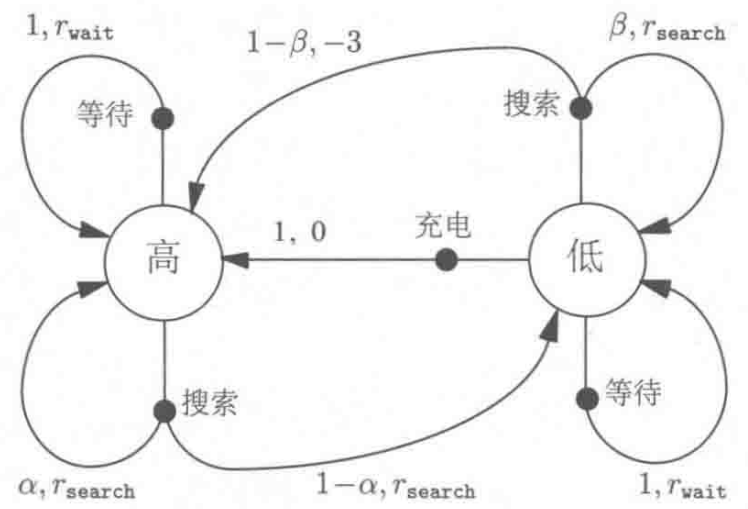
\includegraphics[width=.45\textwidth]{Transitions1}} \quad
\subfloat[状态转移表]{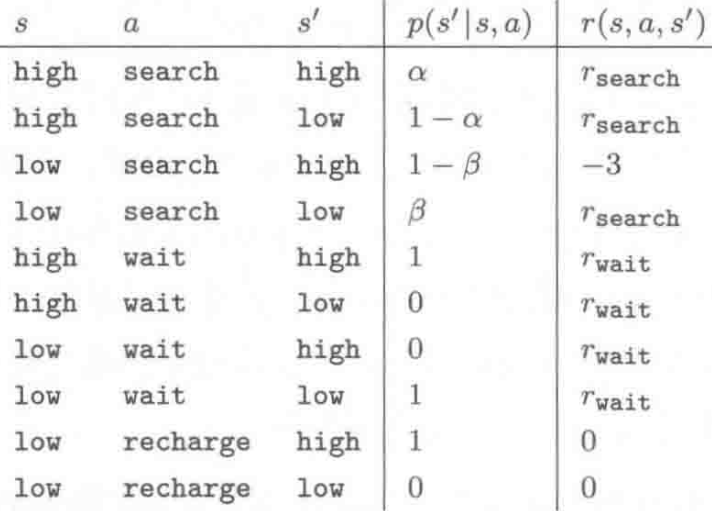
\includegraphics[width=.45\textwidth]{Transitions2}}
\caption[回收机器人状态转移]{回收机器人状态转移}
\end{figure}
%------------------------------------------------
\subsubsection{策略}
%------------------------------------------------
\paragraph{贪婪策略}
$ \pi(a|s) = argmax_a q(a) $。
%------------------------------------------------
\paragraph{探索-利用平衡策略}
\begin{itemize}
\item $ \epsilon $-greedy策略\tip{$ \epsilon $-greedy策略}:
$$
a = 
\begin{cases} 
argmax_a q(a) &, p = 1 - \epsilon \\
random(a) &, p = \epsilon
\end{cases}
\Rightarrow 
\pi(a|s) = 
\begin{cases} 
1 - \epsilon + \frac{\epsilon}{|A|} &, a = argmax_a q(a) \\
\frac{\epsilon}{|A|} &, otherwise
\end{cases}
$$

靠近贪心策略,但所有动作概率不为零。在实际使用时,需要注意多最优情况。
\item UCB(upper confidence bound)策略:
$$ \pi(a|s) = Q(a) + c\sqrt{\frac{\ln N}{n(a)}} $$

其中,$ c $控制探索强度,$ N $是当前轮数,$ n(a) $是$ a $被选次数。

可以自适应平衡探索与利用。
\item 玻尔兹曼分布(Boltzmann):
$$ \pi(a|s) = \frac{e^{Q(a)/\tau}}{\sum_{a'} e^{Q(a)/\tau}} $$

其中$ \tau $是温度参数,控制随机性程度,趋于$ 0 $时接近贪心策略,趋于$ \infty $时接近均匀随机选择。

可以动态调整探索强度。
\item 高斯策略:
$$ \pi = \mu + \epsilon, \epsilon \thicksim N(0, \sigma^2) $$
\end{itemize}
%------------------------------------------------
\paragraph{增量式更新}\tip{增量式更新}
将轮次更新的量化为递推关系,减少空间复杂度,如运行均值:
$$ Q_{n + 1} = \frac{1}{n}\sum_{i = 1}^n R_i = Q_n + \frac{1}{n}(R_n - Q_n) $$
%------------------------------------------------
\subsubsection{回报与折扣}\tip{分幕与回报}
\begin{itemize}
\item 幕(episode):一次交互序列。
\item 分幕式任务:具有分幕重复特性,下一幕开始状态与上一幕终结状态无关。
$$ G_t = R_{t + 1} + R_{t + 2} + \cdots + R_T $$

其中$ T $是最终时刻,由其划分非终结状态集$ S $和所有状态集$ S^+ $。
\item 持续性任务:持续不断发生,不能自然分幕,最终时刻趋于无穷。
$$ G_t = R_{t + 1} + \gamma R_{t + 2} + \gamma^2 R_{t + 3} + \cdots = \sum_{k = 0}^{\infty} \gamma^k R_{t + k + 1} \leq \frac{1}{1 - \gamma}max R_t $$

其中,折扣率$ \gamma \in [0, 1] $越大代表长期收益越重要。
\item 统一表示:有限项终止后,状态持续转移回自己,相当于无限项。
$$ G_t \doteq \sum_{k = t + 1}^{T} \gamma^{k - t - 1} R_k $$
\end{itemize}
%------------------------------------------------
\subsubsection{值函数}\tip{值函数与回溯算法}
%------------------------------------------------
\paragraph{值函数}
\begin{align*}
v_\pi(s) 
&\doteq E_\pi[G_t|S_t = s] = E_\pi[\sum_{k = 0}^{\infty} \gamma^k R_{t + k + 1}|S_t = s], s \in S \\
&= E_\pi[R_{t + 1} + \gamma G_{t+1}|S_t = s] (\text{后继递推关系}) \\
&= \sum_a \pi(a|s) \sum_{s'} \sum_r p(s', r|s, a)\{r + \gamma E_\pi[G_{t + 1}|S_{t + 1} = s']\} (\text{全概率条件期望展开}) \\
&= \underbrace{\sum_a \pi(a|s) \sum_{s', r} p(s', r|s, a)[r + \gamma v_\pi(s')]}_{\text{贝尔曼方程}}
\end{align*}
%------------------------------------------------
\paragraph{行为值函数}
\begin{align*} 
q_\pi(s, a) &\doteq E_\pi[G_t|S_t = s, A_t = a] = E_\pi[\sum_{k = 0}^{\infty} \gamma^k R_{t + k + 1}|S_t = s, A_t = a], s \in S \\
&= R(a|s) + \gamma \sum_{s' \in S} P(a|ss') \sum_{a' \in A} \pi(a'|s')q_{\pi}(s'|a')
\end{align*}

其与值函数有转化关系:
$$ v_\pi(s) = \sum_{a \in A} \pi(a|s) q_\pi(s, a) $$
%------------------------------------------------
\paragraph{回溯算法}~\\
\begin{minipage}{0.3\textwidth}
\hspace{2em}
后继状态的价值信息回传给当前状态。
\end{minipage}
\hfill
\begin{minipage}{0.6\textwidth}
\begin{figure}[H]
\centering 
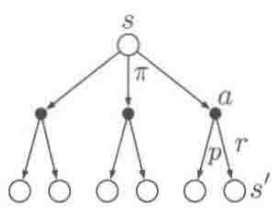
\includegraphics[width=0.5\textwidth]{DP} 
\caption[DP回溯图]{DP回溯图(节点可以重复)}
\end{figure}
\end{minipage}
%------------------------------------------------
\paragraph{最优值函数}~\\

$ \forall s \in S, q_{\pi}(s, \pi'(s)) = v_{\pi'}(s) \geq v_{\pi}(s) $,则称$ \pi' $优于或等于$ \pi $。
值函数定义了策略的偏序关系,最优策略存在且可能不唯一,它们共享最优值函数:
\begin{align*}
v^*(s) &\doteq \max_{\pi} v_{\pi}(s) \\
q^*(s, a) &\doteq \max_{\pi} q_{\pi}(s, a) 
\end{align*}

值函数最优和策略最优等价。
%------------------------------------------------
\subsubsection{构建要点}
\begin{itemize}
\item 确定动作、状态、收益(不含先验知识,不为达到子目标而舍弃最终目标)。
\item 奖励与惩罚:相对的,可以全奖励或全惩罚。
\item 同一问题可能有多层次MDP。
\item 不同状态的可行动作设置:利用先验知识,人为排除愚蠢动作。
\end{itemize}
%----------------------------------------------------------------------------------------
\subsection{贝尔曼方程}\tip{贝尔曼方程}
%------------------------------------------------
\subsubsection{贝尔曼方程}
$$ v_\pi(s) = \sum_a \pi(a|s) \sum_{s', r} p(s', r|s, a) [r + \gamma v_\pi(s')] $$

可化简为$ v = r_\pi + \gamma P_\pi v' $,其说明一个状态依赖其他状态值。
%------------------------------------------------
\subsubsection{贝尔曼最优方程}
方程组中方程数对应状态数,如环境模型$ P $已知,并具有马尔可夫性,则可求解。但一般难以满足,且计算资源有限,求近似解。
%------------------------------------------------
\paragraph{形式}
\begin{itemize}
\item 同一状态,最优动作:转移收益一定,递推最优值函数
\begin{align*}
v_*(s) 
&= \max_{a \in A(s)} q_{\pi_*}(s, a) \\
&= \max_a E[R_{t + 1} + \gamma v_*(S_{t + 1}) | S_t = s, A_t = a] \\
&= \max_a \sum_{s', r} p(s', r|s, a)[r + \gamma v_*(s')]
\end{align*}
\item 统一状态-动作对,最优下一状态-动作对:
\begin{align*}
q_*(s, a) 
&= E[R_{t + 1} + \gamma \max_{a'} q_*(S_{t + 1}, a') | S_t = s, A_t = a] \\
&= \sum_{s', r} p(s', r|s, a)[r + \gamma \max_{a'} q_*(s', a')]
\end{align*}
\end{itemize}

\begin{figure}[H]
\centering 
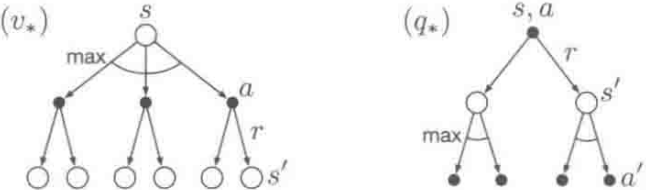
\includegraphics[width=0.7\textwidth]{DPbest} 
\caption[DP回溯图的两种形式(最优)]{DP回溯图的两种形式(最优)}
\end{figure}
%------------------------------------------------
\paragraph{描述方式}
\begin{itemize}
\item 元素:$ v(s) = \max_{\pi} \sum_{s \in S}\pi(a|s)q(s,a) $。
\item 矩阵向量:$ v = \max_{\pi} (r_\pi + \gamma P_\pi v) $。
\end{itemize}
%------------------------------------------------
\paragraph{求解}
伸缩映射性,见\ref{sec:Scalability Mapping}。\label{sec:Scalability Mapping back}
%------------------------------------------------
\paragraph{贪婪最优策略}
最优策略下,各状态价值一定等于其下最优动作的期望回报,可使用贪心策略求取(证明:凸组合最大值为最大一项)。
%----------------------------------------------------------------------------------------
\section{动态规划(Dynamic Programming,DP):期望更新}
\begin{minipage}{0.5\textwidth}
\hspace{2em}
使用值函数结构化组织最优策略搜索,将贝尔曼方程转化成近似逼近理想值函数的递归更新公式,即将多阶段决策问题转化为多个单阶段决策问题。
\end{minipage}
\hfill
\begin{minipage}{0.45\textwidth}
\begin{figure}[H]
\centering 
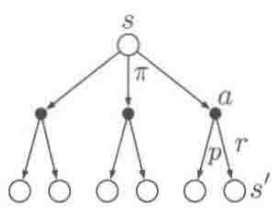
\includegraphics[width=0.6\textwidth]{DP} 
\caption[DP回溯图]{DP回溯图:显示一步的所有转移}
\end{figure}
\end{minipage}
%------------------------------------------------
\subsection{策略迭代}\tip{策略迭代}
反复进行策略评估和策略迭代,得到改进的值函数估计和策略,最后收敛到最优,收敛较快。
%------------------------------------------------
\paragraph{策略评估(PE)}
计算$ v_{\pi_k} $
\begin{itemize}
\item 直接求解:$ v_{\pi_k} = (I - \gamma P_{\pi_k})^{-1} r_{\pi_k} $。
\item 迭代求解:$ v_{\pi_k}^{(j + 1)} = r_{\pi_k} + \gamma P_{\pi_k} v_{\pi_k}^{(j)}, j = 0, 1, 2, \dots $。
\end{itemize}
\begin{enumerate}
\item 期望更新:基于后继可能状态的期望值。
\item 截断策略评估:不需要完全收敛。
\end{enumerate}
%------------------------------------------------
\paragraph{策略改进(PI)}
根据原策略的值函数,利用贪心方法构造新策略,其一定不差于原策略。对于确定性策略和随机策略都成立。
$$ \pi_{k + 1} = argmax_{\pi}(r_{\pi} + \gamma P_{\pi}v_{\pi_k}) $$
%------------------------------------------------
\begin{myalgorithm}[策略迭代]
\State 参数:阈值$ \theta > 0 $确定估计精度
\State 初始化:$ \forall s \in S $,任意初始化$ v(s) \in R, \pi(s) \in A(s) $
\Repeat
\Repeat \Comment{策略评估}
\State $ \Delta \gets 0 $
\For{$ \forall s \in S $}
\State $ v \gets v_{\pi_k}(s) $
\State $ v_{\pi_k}^{(j + 1)}(s) \gets \sum_a \pi_k(a|s)[\sum_r p(r|s,a)r + \gamma \sum_{s'}p(s'|s,a)v_{\pi_k}^{(j)}(s')] $
\State $ \Delta \gets \max(\Delta, |v - v_{\pi_k}^{(j+1)}(s)|) $
\EndFor
\Until{$ \Delta < \theta $}
\State 策略稳定$ \gets $true \Comment{策略改进}
\For{$ \forall s \in S $}
\State $ a_{old} \gets \pi(s) $
\For{$ \forall a \in A(s) $}
\State $ q_{\pi_k}(s,a) \gets \sum_r p(r|s,a)r + \gamma \sum_{s'} p(s'|s,a)v_{\pi_k}(s') $
\EndFor
\State $ \pi(s) \gets argmax_a q_{\pi_k}(s,a) $
\If{$ a_{old} \neq \pi(s) $}
\State 策略稳定$ \gets $false
\EndIf
\EndFor
\Until{策略稳定}
\end{myalgorithm}
%------------------------------------------------
\subsection{值迭代}\tip{值迭代}
只进行一次策略评估遍历,对每个状态更新一次,结合策略改进和极端策略评估。
更新公式如下:
$$ v_{k + 1}(s) = \max_a \sum_{s', r} p(s', r|s, a)[r + \gamma v_k(s')] $$
%------------------------------------------------
\paragraph{策略更新(PU)}
$ \pi_{k + 1} = argmax_{\pi}(r_{\pi} + \gamma P_{\pi}v_k) $,贪婪选取$ a^*_k(s) = argmax_a q_k(a, s) $。
%------------------------------------------------
\paragraph{价值更新(VU)}
$ v_{k + 1} = r_{\pi_{k + 1}} + \gamma P_{\pi_{k + 1}}v_k = max_a q_k(a, s) $。
%------------------------------------------------
\begin{myalgorithm}[值迭代]
\State 参数:阈值$ \theta > 0 $确定估计精度
\State 初始化:$ \forall s \in S^+ $,任意初始化$ v(s) $,其中$ v(\text{终止}) = 0 $
\Repeat
\State $ \Delta \gets 0 $
\For{$ \forall s \in S $}
\State $ v \gets v_k(s) $
\For{$ \forall a \in A(s) $}
\State $ q_k(s, a) \gets \sum_r p(r|s, a)r + \gamma \sum_{s'} p(s'|s, a)v_k(s') $
\EndFor
\State $ a^*_k(s) \gets argmax_a q_k(s, a) $
\State $ v_{k + 1}(s) \gets \max_a q_k(s, a) $
\State 若$ a = a^*_k $且$ \pi_{k + 1}(a|s) = 0 $,则令$ \pi_{k + 1}(a|s) = 1 $
\State $ \Delta \gets \max(\Delta, |v_{k+1}(s) - v|) $
\EndFor
\Until{$ \Delta < \theta $}
\State \Return 策略 $ \pi(s) = argmax_a \sum_{s',r}p(s',r|s,a)[r + \gamma v(s')] $
\end{myalgorithm}
%------------------------------------------------
\subsection{对比}
\begin{itemize}
\item 值迭代:只需要维护值函数,保证收敛到全局最优策略,尤其适用于复杂策略空间,但每次迭代需遍历所有动作,计算成本较高。
\item 策略迭代:需要同时维护值函数和策略,通常比值迭代更快收敛,尤其在策略空间较小时,但依赖初始策略质量,可能陷入局部最优。
\end{itemize}
%------------------------------------------------
\subsection{其他内容}
%------------------------------------------------
\paragraph{异步动态规划}
使用任意可用状态值,以任意顺序更新,避免遍历更新,减小计算量。
%------------------------------------------------
\paragraph{广义策略迭代(GPI)}
策略评估和策略改进以更细粒度进行交替,可视为竞争与合作。
%------------------------------------------------
\paragraph{动态规划的效率}
动态规划的时间复杂度是动作与状态数量的多项式级,在面对维度灾难时,优于线性规划和直接搜索。
%----------------------------------------------------------------------------------------
\section{蒙特卡洛(Monte Carlo,MC):采样更新}\tip{蒙特卡洛}
针对分幕式任务,不需要先验知识,即$ P $,通过多幕采样数据获得经验代替值函数解决问题。
%------------------------------------------------
\subsection{概念}
%------------------------------------------------
\paragraph{核心需求}
由于$ P $的缺失,$ V $是不够的,需要评估$ Q $,即需要对每个状态-动作对进行评估。
%------------------------------------------------
\paragraph{行为值函数估计}
给定的一幕中,指定状态的一次出现叫做对其的一次访问(visit),第一次出现为首次访问。可以不同程度地使用一幕数据。
\begin{itemize}
\item 首次访问(first visit):$ \hat{q}(s) = \frac{G_{11}(s, a) + G_{21}(s, a) + \dots}{N(s, a)} $。
\item 每次访问(every visit):$ \hat{q}(s) = \frac{G_{11}(s, a) + G_{12}(s, a) + \dots + G_{21}(s, a) + \dots}{N(s, a)} $。
\end{itemize}

$ N(s) $是$ s $的访问次数,$ N(s) \to \infty, \hat{q}(s, a) \to q_{\pi}(s, a) $。

\begin{figure}[H]
\centering 
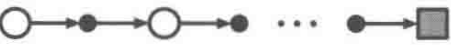
\includegraphics[width=0.3\textwidth]{MC} 
\caption[MC回溯图:显示一幕所有采样到的转移]{MC回溯图:显示一幕所有采样到的转移}
\end{figure}
%------------------------------------------------
\paragraph{幕长}
靠近目标的状态比远离目标的状态更早具有非零值,幕长应足够长,无需无限长。
%------------------------------------------------
\paragraph{优势}
\begin{itemize}
\item 不需要$ P $。
\item 对每个状态的估计是独立的,可聚焦于状态子集,无需考虑其他状态,此时效率很高。
\item 可从实际经历和模拟经历中学习。
\item 无马尔可夫性时性能损失较小。
\end{itemize}
%------------------------------------------------
\subsection{on-policy(同轨)}\tip{on-policy}
采样并改进相同策略,为平衡探索和开发,采用$ \epsilon $-greedy策略。
%------------------------------------------------
\paragraph{试探性出发(ES)}
为采样部分无法正常获得的状态-动作对,可设定所有对都有概率作为起始。满足充分探索的理论要求,但实际中很难实现。
%------------------------------------------------
\begin{myalgorithm}[MC-On-policy(首次访问)]
\State 参数:$ \epsilon > 0 $
\State 初始化:$ \forall s \in S, a \in A(s) $,任意初始化$ Q(s,a) \in R $,初始化$ Returns(s,a) $为空列表,$ \epsilon $-greedy初始化策略$ \pi $
\Loop
\State 根据$ \pi $生成一幕序列$ S_0,A_0,R_1,S_1,A_1,R_2,\dots,S_{T - 1},A_{T - 1},R_T $
\State $ G \gets 0 $
\For{$ t = T - 1, T - 2, \dots, 0 $}
\State $ G \gets \gamma G + R_{t + 1} $
\If{$ S_t $在此幕中首次出现}
\State 将$ G $加入$ Returns(S_t,A_t) $
\State $ Q(S_t,A_t) \gets average[Returns(S_t,A_t)] $
\State $ A^* \gets argmax_a Q(S_t,a) $
\State $ \epsilon $-greedy策略选取$ \pi(a|S_t) $
\EndIf
\EndFor
\EndLoop
\end{myalgorithm}
%------------------------------------------------
\subsection{off-policy(离轨)}\tip{off-policy}
采样与改进不同策略,前者称为行为策略(Behavior Policy)$ b $(保证对所有可能动作的采样),后者称为目标策略(Target Policy)$ \pi $,可视为特殊的离轨。
%------------------------------------------------
\paragraph{重要度采样(importance sampling)}\tip{重要度采样}~\\

计算回报时,对轨迹在目标策略和行为策略中出现的相对概率进行加权:
$$ \rho_{t:T - 1} = \Pi_{k = t}^{T - 1} \frac{\pi(A_k|S_k)}{b(A_k|S_k)} \text{(约去相同的转移概率)} $$
\begin{itemize}
\item 普通重要度采样:$ V(s) \doteq \frac{\sum_{t \in \tau(s)} \rho_{t:T(t) - 1}G_t}{|\tau(s)|} $,无偏但无界。
\item 加权重要度采样:$ V(s) \doteq \frac{\sum_{t \in \tau(s)} \rho_{t:T(t) - 1}G_t}{\sum_{t \in \tau(s)} \rho_{t:T(t) - 1}} $,有偏但偏差值渐近收敛。
\end{itemize}

减小方差的方法:
\begin{itemize}
\item 折扣敏感:把折扣率$ \gamma $视作幕终止的概率,得到第$ n $步终止的无折扣部分回报$ \sum_{i = 1}^n R_{t + i} $,即平价部分回报。全回报$ G_t = \sum_{i = 1}^{T - t} \gamma^{i - 1}R_{t + i} $可视为各平价部分回报的加权和,即该步截止得到的回报与概率之积的和。适用于普通型和加权型。
\item 每次决策型:$ E[\rho_{t:T - 1}G_t] = E[\tilde{G_t}] = E[\sum_{i = 1}^{T - t} \gamma^{i - 1} \rho_{t:t + i - 1}R_{t + i}] $。适用于普通型。
\end{itemize}
%------------------------------------------------
\paragraph{增量式更新}
\begin{align*}
V_{n + 1} &\doteq V_n + \frac{W_n}{C_n}[G_n - V_n] \\
C_{n + 1} &\doteq C_n + W_{n + 1}
\end{align*}

其中,$ W_i $是随机权重,$ C_i $是其累加和。
%------------------------------------------------
\begin{myalgorithm}[MC-Off-policy(每次访问)]
\State 初始化:$ \forall s \in S, a \in A(s) $,任意初始化$ Q(s,a) \in R, C(s,a) = 0 $,初始化$ \pi(s) = argmax_a Q(s,a) $ \Comment{目标策略为贪心策略}
\Loop
\State 根据$ b $生成一幕序列$ S_0,A_0,R_1,S_1,A_1,R_2,\dots,S_{T - 1},A_{T - 1},R_T $ \Comment{行为策略为$ \epsilon $-greedy策略}
\State $ G \gets 0, W \gets 1 $
\For{$ t = T - 1, T - 2, \dots, 0 $}
\State $ G \gets \gamma G + R_{t + 1} $
\State $ C(S_t,A_t) \gets C(S_t,A_t) + W $
\State $ Q(S_t,A_t) \gets Q(S_t,A_t) + \frac{W}{C(S_t,A_t)}[G - Q(S_t,A_t)] $
\State $ \pi(S_t) \gets argmax_a Q(S_t,a) $
\If{$ A_t \neq \pi(S_t) $}
\State break \Comment{如果不是最优动作则退出内层循环}
\EndIf
\State $ W \gets W \cdot \frac{1}{b(A_t|S_t)} $ \Comment{更新重要度采样权重}
\EndFor
\EndLoop
\end{myalgorithm}

潜在问题:贪心行为普遍时,只会从幕尾学习;贪心行为不普遍时,学习速度较慢。
%------------------------------------------------
\subsection{对比}
\begin{itemize}
\item on-policy通常具有更高的稳定性,但可能需要更多样本才能收敛,因为每次策略更新后都需要新的数据。
\item off-policy虽然可能更快找到好的解,但由于使用了不同的行为策略,学习过程可能不太稳定。
\end{itemize}
%----------------------------------------------------------------------------------------
\section{时序差分(Temporal Difference,TD):采样更新}
TD可直接从与环境的互动中获取信息,不需要$ P $,同时运用自举思想,可基于已得到的其他状态估计来更新当前$ v(s) $,相当于结合了DP和MC的优点。
%------------------------------------------------
\subsection{TD($ 0 $)}\tip{时序差分(TD($ 0 $))}
TD($ 0 $)的更新公式为:
$$ V_{t + 1}(S_t) = V_t(S_t) + \alpha_t(S_t)[R_{t + 1} + \gamma V_t(S_{t + 1}) - V_t(S_t)] $$
\begin{itemize}
\item TD误差$ \delta_t = R_{t + 1} + \gamma V_t(S_{t + 1}) - V_t(S_t) $。
\item TD目标$ R_{t + 1} + \gamma V_t(S_{t + 1}) $
\end{itemize}

MC误差可写成TD误差之和$ G_t - V(S_t) = \sum_{k = t}^{T - 1} \gamma^{k - t} \delta_k $,其在步长较小时成立。

\begin{figure}[H]
\centering
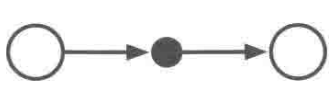
\includegraphics[width=0.2\textwidth]{TD}
\caption[TD回溯图]{TD回溯图}
\end{figure}
%------------------------------------------------
\paragraph{优势}
\begin{itemize}
\item 不需要$ P,R $。
\item 更新快:MC须等到幕尾确定增量,更新$ G_t $;而TD只需等到下一时刻,更新TD目标。
\item 只评估当前动作,与后续动作无关。
\end{itemize}
%------------------------------------------------
\begin{myalgorithm}[TD($ 0 $)]
\State 输入:待评估策略$ \pi $
\State 参数:步长$ \alpha \in (0,1] $
\State 初始化:$ \forall s \in S^+ $,任意初始化$ V(s), V(\text{终止状态}) = 0 $
\For{每一幕}
\State 初始化$ S $
\While{$ S $不是终止状态}
\State $ A \gets \pi(S) $
\State 执行动作$ A $,观察$ R, S' $
\State $ V(S) \gets V(S) + \alpha[R + \gamma V(S') - V(S)] $
\State $ S \gets S' $
\EndWhile
\EndFor
\end{myalgorithm}
%------------------------------------------------
\paragraph{随机游走}
在随机任务实践中,TD($ 0 $)的收敛速度要比常量$ \alpha $MC快。这是因为前者的最优性与预测回报更相关,找出的是完全符合马尔可夫过程模型的最大似然估计参数,收敛到确定性等价估计;而后者只在有限方面最优,找出的是最小化训练集均方误差的估计。
%------------------------------------------------
\paragraph{批量更新}
值函数根据增量和改变,在处理整批数据后才更新。
%------------------------------------------------
\subsection{Sarsa(on-policy-TD)}\tip{Sarsa(on-policy-TD)}
Sarsa(State-Action-Reward-State-Action)是TD算法的行为值函数版本:
$$ Q_{t + 1}(S_t, A_t) = Q_t(S_t, A_t) + \alpha_t[R_{t + 1} + \gamma Q_t(S_{t + 1}, A_{t + 1}) - Q_t(S_t, A_t)] $$

\begin{figure}[H]
\centering
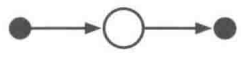
\includegraphics[width=0.2\textwidth]{Sarsa}
\caption[Sarsa回溯图]{Sarsa回溯图}
\end{figure}
%------------------------------------------------
\begin{myalgorithm}[Sarsa(on-policy-TD)]
\State 参数:步长$ \alpha \in (0,1], \epsilon > 0 $
\State 初始化:$ \forall s \in S^+ $,任意初始化$ Q(s,a), Q(\text{终止状态}, \cdot) = 0 $
\For{每一幕}
\State 初始化$ S $
\State 使用从$ Q $得到的$ \epsilon $-greedy策略,在$ S $处选择$ A $
\While{$ S $不是终止状态}
\State 执行动作$ A $,观察$ R,S' $
\State 使用从$ Q $得到的$ \epsilon$-greedy策略,在$ S' $处选择$ A' $
\State $ Q(S, A) \gets Q(S, A) + \alpha [R + \gamma Q(S', A') - Q(S, A)] $
\State $ S \gets S', A \gets A' $
\EndWhile
\EndFor
\end{myalgorithm}
%------------------------------------------------
\paragraph{期望Sarsa}\tip{期望Sarsa}
$$ Q_{t + 1}(S_t, A_t) = Q_t(S_t, A_t) + \alpha_t[R_{t + 1} + \gamma \sum_a \pi(a|S_{t + 1}) Q_t(S_{t + 1}, a) - Q_t(S_t, A_t)] $$

\begin{minipage}{0.6\textwidth}
\hspace{2em}
期望Sarsa相较Sarsa,虽然计算复杂,但是消除了随机选择带来的方差。$ \alpha $的选择对二者有一定影响,尤其在长期稳态性能上。生成策略可以基于相同或不同策略,即离轨或在轨是可变的。基于此,Q-learning可视为期望Sarsa的一个特例。
\end{minipage}
\hfill
\begin{minipage}{0.35\textwidth}
\begin{figure}[H]
\centering
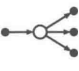
\includegraphics[width=0.5\textwidth]{eSarsa}
\caption[期望Sarsa回溯图]{期望Sarsa回溯图}
\end{figure}
\end{minipage}
%------------------------------------------------
\subsection{Q-learning(off-policy-TD)}\tip{Q-learning(off-policy-TD)}
Q-learning旨在求解行为值贝尔曼最优方程,直接逼近$ q^*(s, a) $。
$$ Q_{t + 1}(S_t, A_t) = Q_t(S_t, A_t) + \alpha_t[R_{t + 1} + \gamma \max_a Q_t(S_{t + 1}, a) - Q_t(S_t, A_t)] $$

\begin{figure}[H]
\centering
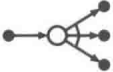
\includegraphics[width=0.2\textwidth]{Q}
\caption[Q-learning回溯图]{Q-learning回溯图}
\end{figure}
%------------------------------------------------
\begin{myalgorithm}[Q-learning(off-policy-TD)]
\State 参数:步长$ \alpha \in (0,1] $,探索率$ \epsilon > 0 $
\State 初始化:$ \forall s \in S^+, a \in A(s) $,任意初始化$ Q(s,a), Q(\text{终止状态}, \cdot) = 0 $
\For{每一幕}
\State 初始化$ S $
\While{$ S $不是终止状态}
\State 使用从$ Q $得到的$ \epsilon $-greedy策略,在$ S $处选择$ A $
\State 执行动作$ A $,观察$ R,S' $
\State $ Q(S, A) \gets Q(S, A) + \alpha [R + \gamma \max_a Q(S', a) - Q(S, A)] $
\State $ S \gets S' $
\EndWhile
\EndFor
\end{myalgorithm}
%------------------------------------------------
\paragraph{双Q-learning}\tip{双Q-learning}
$$ Q_{1_{t + 1}}(S_t, A_t) = Q_{1_t}(S_t, A_t) + \alpha_t\{R_{t + 1} + \gamma Q_{2_t}[S_{t + 1}, argmax_a Q_{1_t}(S_{t + 1}, a)] - Q_{1_t}(S_t, A_t)\} $$
\begin{figure}[H]
\centering
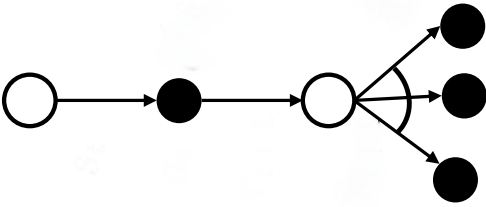
\includegraphics[width=0.2\textwidth]{dQ}
\caption[双Q-learning回溯图]{双Q-learning回溯图}
\end{figure}

\begin{itemize}
\item 最大化偏差:贪心策略和柔性策略都在隐式估计最大值,会产生正偏差,致使回报值偏离,带来明显错误决策。
\item 双学习:划分样本,学习两个独立的估计$ Q_1(a),Q_2(a) $,确定动作$ A* = argmax_a Q_1(a) $,再计算价值的估$ Q_2(A*) = Q_2(argmax_a Q_1(a)) $,后者是无偏的(可以交换再来一次)。需要双倍内存,但是计算量维持。
\item 后位状态:利用先验知识,知晓动作后状态,并有后位值函数。在后位状态相同的时候可以迁移,减少计算量。
\end{itemize}
%------------------------------------------------
\begin{myalgorithm}[双Q-learning]
\State 参数:步长$ \alpha \in (0,1] $,探索率$ \epsilon > 0 $
\State 初始化:$ \forall s \in S^+, a \in A(s) $,任意初始化$ Q_1(s,a),Q_2(s,a), Q_1(\text{终止状态}, \cdot) = Q_2(\text{终止状态}, \cdot) = 0 $
\For{每一幕}
\State 初始化$ S $
\While{$ S $不是终止状态}
\State 基于$ Q_1 + Q_2 $,使用$ \epsilon $-greedy策略在$ S $处选择$ A $
\State 执行动作$ A $,观察$ R,S' $
\If{以$ 0.5 $的概率}
\State $ Q_1(S, A) \gets Q_1(S, A) + \alpha [R + \gamma Q_2(S', argmax_a Q_1(S',a)) - Q_1(S, A)] $
\Else
\State $ Q_2(S, A) \gets Q_2(S, A) + \alpha [R + \gamma Q_1(S', argmax_a Q_2(S',a)) - Q_2(S, A)] $
\EndIf
\State $ S \gets S' $
\EndWhile
\EndFor
\end{myalgorithm}
%------------------------------------------------
\subsection{对比}
Sarsa较为保守,在存在风险的任务中,会避开低回报动作; Q-learning较为乐观,更倾向于探索并找到最优解。在存在陷阱的任务中,Sarsa会比Q-learning取得更好的结果。
%----------------------------------------------------------------------------------------
\section{n步自举法}
%------------------------------------------------
\subsection{n-TD}\tip{n-TD}
n-TD作为MC和TD的一般推广,在两种极端方法间找到了性能更好的平衡点。n-TD在$ n $步后进行更新,截断得到$ n $步回报。
$$ G_{t:t + n} \doteq R_{t + 1} + \gamma R_{t + 2} + \dots + \gamma^{n - 1} R_{t + n} + \gamma^n V_{t + n - 1}(S_{t + n}) $$

其中$ V_{t + n}(S_t) \doteq V_{t + n - 1}(S_t) + \alpha[G_{t:t + n} - V_{t + n - 1}(S_t)] $。
%------------------------------------------------
\begin{myalgorithm}[n-TD]
\State 输入:待评估策略$ \pi $
\State 参数:步长$ \alpha \in (0,1], n \in N_+ $
\State 初始化:$ \forall s \in S $,任意初始化$ V(s) $
\For{每一幕}
\State 初始化$ S_0 $为非终止状态
\State $ T \gets \infty $
\For{$ t = 0, 1, 2, \dots $}
\If{$ t < T $}
\State 根据$ \pi(\cdot|S_t) $采取动作$ A_t $
\State 观察$ R_{t + 1},S_{t + 1} $
\If{$ S_{t + 1} $是终止状态}
\State $ T \gets t + 1 $
\EndIf
\EndIf
\State $ \tau \gets t - n + 1 $ \Comment{$ \tau $是正在更新的状态的时间}
\If{$ \tau \geq 0 $}
\State $ G \gets \sum_{i = \tau + 1}^{\min(\tau + n,T)} \gamma^{i - \tau - 1}R_i $
\If{$ \tau + n < T $}
\State $ G \gets G + \gamma^n V(S_{\tau + n}) $
\EndIf
\State $ V(S_{\tau}) \gets V(S_{\tau}) + \alpha[G - V(S_{\tau})] $
\EndIf
\If{$ \tau = T - 1 $}
\State break
\EndIf
\EndFor
\EndFor
\end{myalgorithm}
%------------------------------------------------
\subsection{n-Sarsa}\tip{n-Sarsa}
n-Sarsa统一了Sarsa和MC,其节点转移全部基于采样得到的单独路径:
$$ Q_{t + n}(S_t, A_t) \doteq Q_{t + n - 1}(S_t, A_t) + \alpha [G_{t:t + n} - Q_{t + n - 1}(S_t, A_t)] $$

n-期望Sarsa只对最后一个状态到动作的转移展开:
$$ G_{t:t + n} \doteq R_{t + 1} + \gamma R_{t + 2} + \dots + \gamma^{n - 1} R_{t + n} + \gamma^n \bar{V}_{t + n - 1}(S_{t + n}) $$

\begin{figure}[H]
\centering
\subfloat[n-Sarsa]{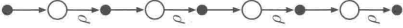
\includegraphics[width=.6\textwidth]{nSarsa}} \\
\subfloat[n-期望Sarsa]{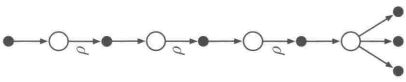
\includegraphics[width=.6\textwidth]{neSarsa}}
\caption[n-Sarsa回溯图]{n-Sarsa回溯图}
\end{figure}
%------------------------------------------------
\begin{myalgorithm}[n-Sarsa]
\State 参数:步长$ \alpha \in (0,1] $,探索率$ \epsilon > 0 $,步数$ n \in N_+ $
\State 初始化:$ \forall s \in S, a \in A $,任意初始化$ Q(s, a) $,初始化$ \pi $(如基于$ Q $的$ \epsilon $-greedy策略)
\For{每一幕}
\State 初始化$ S_0 $为非终止状态
\State 根据$ \pi(\cdot|S_0) $选取$ A_0 $
\State $ T \gets \infty $
\For{$ t = 0, 1, 2, \dots $}
\If{$ t < T $}
\State 执行动作$ A_t $,观察$ R_{t + 1},S_{t + 1} $
\If{$ S_{t + 1} $是终止状态}
\State $ T \gets t + 1 $
\Else
\State 根据$ \pi(\cdot|S_{t + 1}) $选取$ A_{t + 1} $
\EndIf
\EndIf
\State $ \tau \gets t - n + 1$ \Comment{$ \tau $是正在更新的状态的时间}
\If{$ \tau \geq 0 $}
\State $ G \gets \sum_{i = \tau + 1}^{\min(\tau + n,T)} \gamma^{i - \tau - 1}R_i $
\If{$ \tau + n < T $}
\State $ G \gets G + \gamma^n Q(S_{\tau + n}, A_{\tau + n}) $
\EndIf
\State $ Q(S_{\tau}, A_{\tau}) \gets Q(S_{\tau}, A_{\tau}) + \alpha[G - Q(S_{\tau}, A_{\tau})] $
\EndIf
\If{$ \tau = T - 1 $}
\State break
\EndIf
\EndFor
\EndFor
\end{myalgorithm}
%------------------------------------------------

针对离线n步时序差分学习有:
$$ V_{t + n}(S_t) \doteq V_{t + n - 1}(S_t) + \alpha \rho_{t:t + n - 1}[G_{t:t + n} - V_{t + n - 1}(S_t)] $$

其中,重要度采样率为目标策略和行为策略采取$ n $个动作的相对概率:
$$ \rho_{t:h} \doteq \prod_{k = t}^{\min(h, T - 1)} \frac{\pi(A_k|S_k)}{b(A_k|S_k)} $$
%------------------------------------------------
\begin{myalgorithm}[n-期望Sarsa-off-policy]
\State 输入:行为策略$ b $,满足$ b(a|s) > 0 $
\State 参数:步长$ \alpha \in (0,1] $,探索率$ \epsilon > 0 $,步数$ n \in N_+ $
\State 初始化:$ \forall s \in S, a \in A $,任意初始化$ Q(s, a) $,初始化目标策略$ \pi $
\For{每一幕}
\State 初始化$ S_0 $为非终止状态
\State 根据$ b(\cdot|S_0) $选取$ A_0 $
\State $ T \gets \infty $
\For{$ t = 0, 1, 2, \dots $}
\If{$ t < T $}
\State 执行动作$ A_t $,观察$ R_{t + 1},S_{t + 1} $
\If{$ S_{t + 1} $是终止状态}
\State $ T \gets t + 1 $
\Else
\State 根据 $ b(\cdot|S_{t + 1}) $选取$A_{t + 1} $
\EndIf
\EndIf
\State $ \tau \gets t - n + 1 $ \Comment{$ \tau $是正在更新的状态的时间}
\If{$ \tau \geq 0 $}
\State $ \rho \gets \prod_{i = \tau + 1}^{\min(\tau + n - 1,T - 1)} \frac{\pi(A_i|S_i)}{b(A_i|S_i)}$ \Comment{重要性采样权重}
\State $ G \gets \sum_{i = \tau + 1}^{\min(\tau + n,T)} \gamma^{i - \tau - 1}R_i $
\If{$ \tau + n < T $}
\State $ G \gets G + \gamma^n \sum_a\pi(a|S_{\tau + n})Q(S_{\tau + n}, a)$ \Comment{期望Sarsa使用期望值}
\EndIf
\State $ Q(S_{\tau}, A_{\tau}) \gets Q(S_{\tau}, A_{\tau}) + \alpha \rho[G - Q(S_{\tau}, A_{\tau})] $
\EndIf
\If{$ \tau = T - 1 $}
\State break
\EndIf
\EndFor
\EndFor
\end{myalgorithm}
%------------------------------------------------
\subsection{n-树回溯}\tip{n-树回溯}
%------------------------------------------------
\paragraph{带控制变量的每次决策模型}~\\

为保证不被选择的动作不会因$ \rho_t = 0 $而回报为$ 0 $,使方差较大,采取以下n步回报off-policy方法:
$$ G_{t:h} \doteq \rho_t (R_{t + 1} + \gamma G_{t + 1:h}) + (1 - \rho_t) V_{h - 1}(S_t) $$

其中$ (1 - \rho_t) V_{h - 1}(S_t) $称为控制变量,其能保证$ \rho_t = 0 $时估计值不收缩,但不会改变更新值的期望。

可写为以下递归形式:
\begin{align*}
G_{t:h} 
&\doteq R_{t + 1} + \gamma[\rho_{t + 1} G_{t + 1:h} + \bar{V}_{h - 1}(S_{t + 1}) - \rho_{t + 1} Q_{h - 1}(S_{t + 1}, A_{t + 1})] \\
&= R_{t + 1} + \gamma \rho_{t + 1}[G_{t + 1:h} - Q_{h - 1}(S_{t + 1}, A_{t + 1})] + \gamma \bar{V}_{h - 1}(S_{t + 1})
\end{align*}
%------------------------------------------------
\paragraph{n-树回溯}~\\

off-policy因所学内容相关性小,比on-policy慢,一些方法可以缓解这一问题,比如不使用重要度采样的树回溯算法。相比于前面以沿途收益和底部节点估计价值为更新目标的算法,树回溯的更新源于整个树的行为值估计,即各叶子节点的行为值估计按出现概率加权。
单步回溯树:
$$ G_{t:t + 1} \doteq R_{t + 1} + \gamma \sum_{a} \pi(a|S_{t + 1}) Q_t(S_{t + 1}, a) $$

拓展到n-回溯树的递归形式,其对路径可能分支进行展开,不进行采样:
$$ G_{t:t + n} \doteq R_{t + 1} + \gamma \sum_{a \neq A_{t + 1}} \pi(a|S_{t + 1}) Q_{t + n - 1}(S_{t + 1}, a) + \gamma \pi(A_{t + 1}|S_{t + 1}) G_{t + 1:t + n} $$

\begin{figure}[H]
\centering
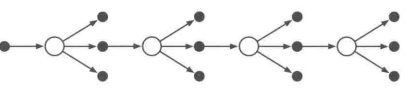
\includegraphics[width=0.6\textwidth]{ntree}
\caption[n-树回溯回溯图]{n-树回溯回溯图}
\end{figure}
%------------------------------------------------
\begin{myalgorithm}[n-树回溯]
\State 参数:步长$ \alpha \in (0,1], n \in N_+ $
\State 初始化:$ \forall s \in S, a \in A $,任意初始化$ Q(s, a) $,初始化$ \pi $
\For{每一幕}
\State 初始化$ S_0 $为非终止状态
\State 根据$ S_0 $任意选取$ A_0 $
\State $ T \gets \infty $
\For{$ t = 0, 1, 2, \dots $}
\If{$ t < T $}
\State 执行动作$ A_t $,观察$ R_{t + 1},S_{t + 1} $
\If{$ S_{t + 1} $是终止状态}
\State $ T \gets t + 1 $
\Else
\State 根据$ S_{t + 1} $选取$ A_{t + 1} $
\EndIf
\EndIf
\State $ \tau \gets t - n + 1 $ \Comment{$ \tau $是正在更新的状态的时间}
\If{$ \tau \geq 0 $}
\If{$ t + 1 \geq T $}
\State $ G \gets R_T $ 
\Else
\State $ G \gets R_{t + 1} + \gamma \sum_a \pi(a|S_{t + 1})Q(S_{t + 1}, a) $
\EndIf
\For{$ k = \min(t, T - 1) $递减到$ \tau + 1 $}
\State $ G \gets R_k + \gamma \sum_{a \neq A_k} \pi(a|S_k)Q(S_k,a) + \gamma \pi(A_k|S_k)G $
\EndFor
\State $ Q(S_{\tau}, A_{\tau}) \gets Q(S_{\tau}, A_{\tau}) + \alpha[G - Q(S_{\tau}, A_{\tau})] $
\EndIf
\If{$ \tau = T - 1 $}
\State break
\EndIf
\EndFor
\EndFor
\end{myalgorithm}
%------------------------------------------------
\subsection{n-Q($ \sigma $)}\tip{n-Q($ \sigma $)}
结合采样的Sarsa和展开的树回溯,在每个状态由参数$ \sigma $决定是采样还是展开,将两种线性情况组合起来:
$$ G_{t:h} \doteq R_{t + 1} + \gamma (\sigma_{t + 1} \rho_{t + 1} + (1 - \sigma_{t + 1}) \pi(A_{t + 1}|S_{t + 1}))(G_{t + 1:h} - Q_{h - 1}(S_{t + 1}, A_{t + 1})) + \gamma \bar{V}_{h - 1}(S_{t + 1}) $$

\begin{figure}[H]
\centering
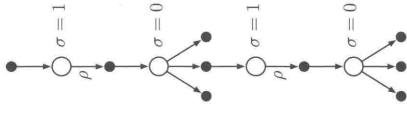
\includegraphics[width=0.6\textwidth]{Qsigma}
\caption[Q(sigma)回溯图]{Q(sigma)回溯图}
\end{figure}
%------------------------------------------------
\begin{myalgorithm}[n-Q($ \sigma $)-off-policy]
\State 输入:行为策略$ b $,满足$ b(a|s) > 0 $
\State 参数:步长$ \alpha \in (0,1] $,探索率$ \epsilon > 0 $,步数$ n \in N_+ $
\State 初始化:$ \forall s \in S, a \in A $,任意初始化$ Q(s, a) $,初始化目标策略$ \pi $
\For{每一幕}
\State 初始化$ S_0 $为非终止状态
\State 根据$ b(\cdot|S_0) $选取$ A_0 $
\State $ T \gets \infty $
\For{$ t = 0, 1, 2, \dots $}
\If{$ t < T $}
\State 执行动作$ A_t $,观察$ R_{t + 1},S_{t + 1} $
\If{$ S_{t + 1} $是终止状态}
\State $ T \gets t + 1 $
\Else
\State 根据$ b(\cdot|S_{t + 1}) $选取$ A_{t + 1} $
\State 选择$ \sigma_{t + 1} $ \Comment{指示是采样还是展开}
\State $ \rho_{t + 1} \gets \frac{\pi(A_{t + 1}|S_{t + 1})}{b(A_{t + 1}|S_{t + 1})}$ \Comment{重要性采样比率}
\EndIf
\EndIf
\State $ \tau \gets t - n + 1 $ \Comment{$ \tau $是正在更新的状态的时间}
\If{$ \tau \geq 0 $}
\State $ G \gets 0 $
\For{$ k = \min(t, T - 1) $递减到$ \tau + 1 $}
\If{$ k = T $}
\State $ G \gets R_T $
\Else
\State $ \bar{V} \gets \sum_a \pi(a|S_k)Q(S_k, a) $ \Comment{计算期望状态值}
\State $ G \gets R_k + \gamma[\sigma_k \rho_k + (1 - \sigma_k)\pi(A_k|S_k)][G - Q(S_k,A_k)] + \gamma\bar{V} $
\EndIf
\EndFor
\State $ Q(S_{\tau},A_{\tau}) \gets Q(S_{\tau},A_{\tau}) + \alpha[G - Q(S_{\tau},A_{\tau})] $
\EndIf
\If{$ \tau = T - 1 $}
\State break
\EndIf
\EndFor
\EndFor
\end{myalgorithm}
%----------------------------------------------------------------------------------------
\section{表格型方法总结对比}\tip{表格型方法总结对比}
基于模型的方法(DP、启发式搜索)主要进行规划,无模型的方法(MC、TD)主要进行学习,二者的核心都是值函数的计算。
%------------------------------------------------
\paragraph{表格型方法介绍}\label{sec:table back}
见\ref{sec:table}
%------------------------------------------------
\paragraph{三个维度}~\\
\begin{minipage}{0.3\textwidth}
\begin{itemize}
\item 更新
\item 自举程度
\item 同轨/离轨
\end{itemize}
\end{minipage}
\hfill
\begin{minipage}{0.6\textwidth}
\begin{figure}[H]
\centering
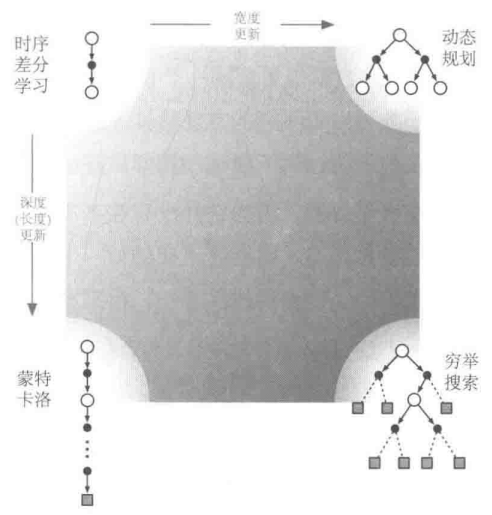
\includegraphics[width=0.8\textwidth]{all}
\caption[表格型方法总结对比]{表格型方法总结对比}
\end{figure}
\end{minipage}
%------------------------------------------------
\paragraph{更新}
期望更新能产生更好的估计,但是需要更多的计算。

\begin{figure}[H]
\centering
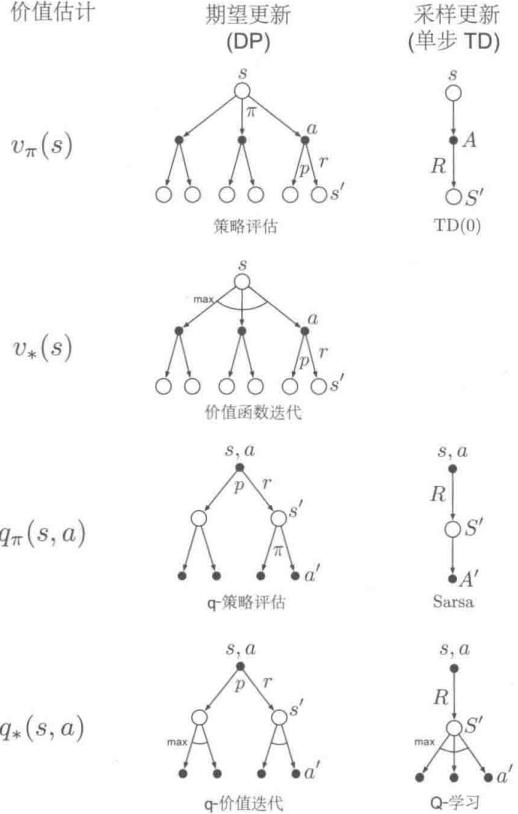
\includegraphics[width=0.5\textwidth]{compare_update}
\caption[表格型方法更新对比]{更新对比}
\end{figure}
%------------------------------------------------
\paragraph{表达式对比}
\begin{figure}[H]
\centering
\subfloat[DP]{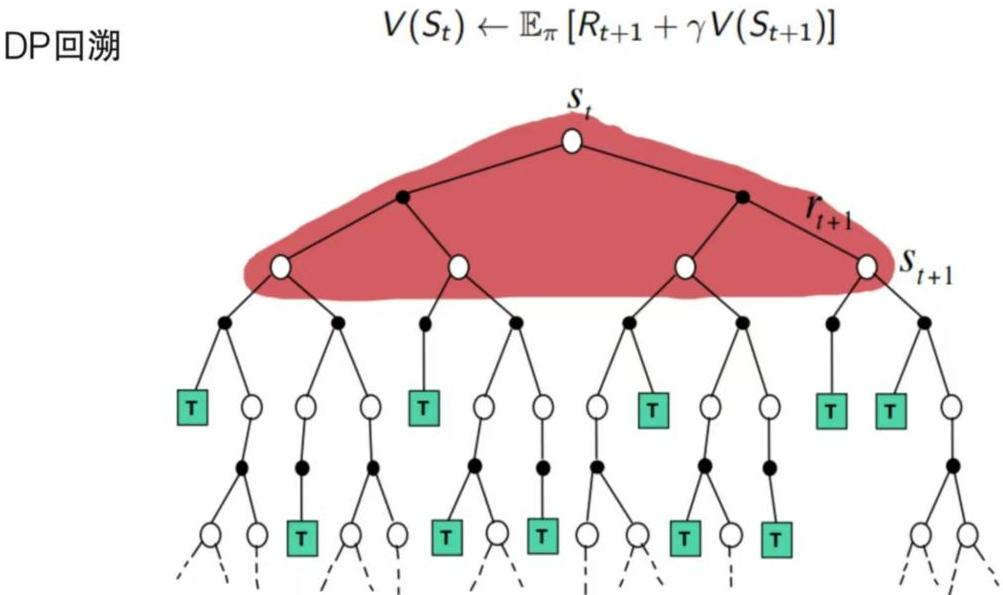
\includegraphics[width=.3\textwidth]{compare_DP}} \quad
\subfloat[MC]{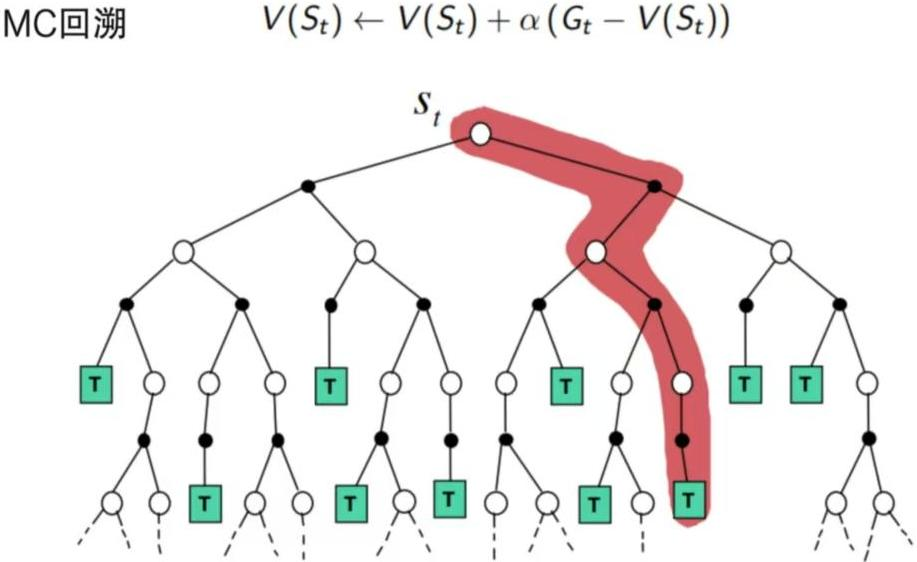
\includegraphics[width=.3\textwidth]{compare_MC}} \quad
\subfloat[TD]{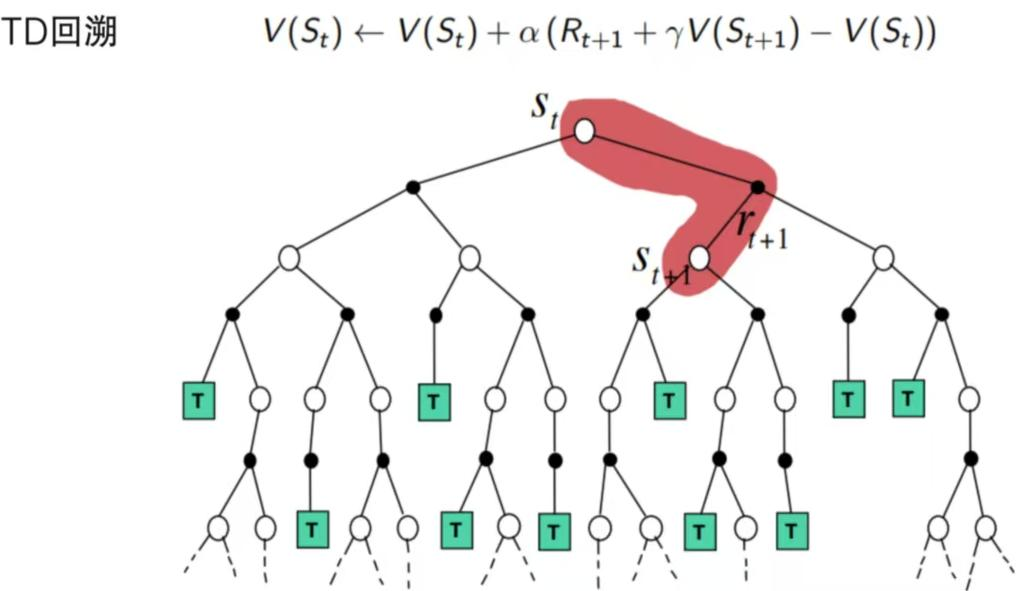
\includegraphics[width=.3\textwidth]{compare_TD}}
\caption[表达式对比]{表达式对比}
\end{figure}

统一格式:
$$ Q_{t + 1}(S_t, A_t) = Q_t(S_t, A_t) + \alpha_t(S_t, A_t)[\bar{q}_t - Q_t(S_t, A_t)] $$

\begin{figure}[H]
\centering
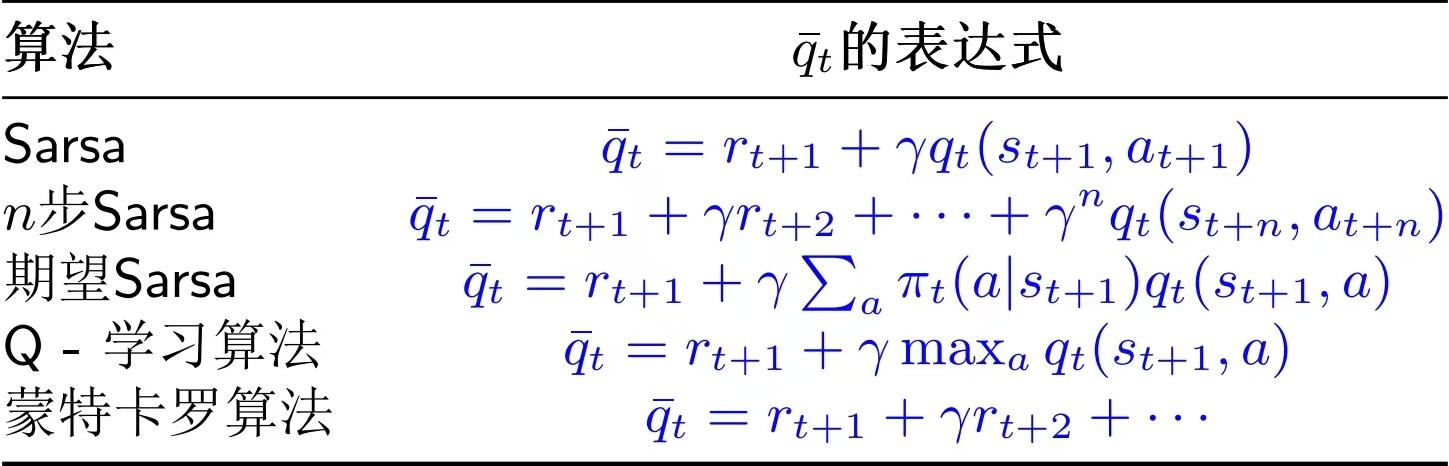
\includegraphics[width=0.6\textwidth]{all_q}
\caption[表达式对比]{表达式对比}
\end{figure}
%----------------------------------------------------------------------------------------
\section{值函数近似}
%------------------------------------------------
\subsection{函数近似}
$$ \hat{v}(s, w) \approx v_{\pi}(s), w \in R^d, d \ll |S| $$
%------------------------------------------------
\paragraph{目标函数}
$$ J(\omega) = E[(v_{\pi}(S) - \hat{v}(S, \omega))^2] $$

在对状态按重要程度进行加权后,可得到均方值误差:
$$ \overline{VE} (w) \doteq \sum_{s \in S} \mu(s) [v_\pi(s) - \hat{v}(s, w)]^2 $$

一般无法保证最优,求解局部最优。
%------------------------------------------------
\paragraph{状态分布}
\begin{itemize}
\item 均匀分布(各状态同等重要):$ J(\omega) = \frac{1}{|S|}\sum_{s \in S}[v_{\pi}(s) - \hat{v}(s, \omega)]^2 $。
\item 平稳分布(马氏过程长期行为):$ J(\omega) = \sum_{s \in S}d_{\pi}(s)[v_{\pi}(s) - \hat{v}(s, \omega)]^2 $。
\end{itemize}
%------------------------------------------------
\paragraph{优势}
\begin{itemize}
\item 具有一定泛化能力,适应部分观测问题。
\item 曲线拟合:用少量参数储存状态,阶数越高越近似。
\end{itemize}
%------------------------------------------------
\subsection{随机梯度下降(SGD)}\tip{随机梯度下降}
$$ \omega_{k + 1} = \omega_k - \alpha_k \nabla_\omega J(\omega_k) $$

其中,
\begin{align*}
\nabla_\omega J(\omega)
&= \nabla_\omega E[(v_\pi(S) - \hat{v}(S, \omega))^2] \\
&= E[\nabla_\omega (v_\pi(S) - \hat{v}(S, \omega))^2] (\text{有界可换求导与期望顺序}) \\
&= -2E[(v_\pi(S) - \hat{v}(S, \omega)) \nabla_\omega \hat{v}(S, \omega)]
\end{align*}

因此$ \omega_{k + 1} = \omega_k + \alpha (v_\pi(s_k) - \hat{v}(s_k, \omega_k)) \nabla_\omega \hat{v}(s_k, \omega_k) $。
%------------------------------------------------
\paragraph{负梯度方向降速最快}
梯度方向增长最快,负梯度方向下降最快。
%------------------------------------------------
\paragraph{步长$ \alpha $}
%------------------------------------------------
\paragraph{近似方法}\label{sec:kernal back}
\begin{itemize}
\item $ v_\pi(s_t) $:
\begin{itemize}
\item 蒙特卡洛:$ g_t $。
\item 时序差分:$ r_{t + 1} + \gamma \hat{v}(s_{t + 1}, \omega_t) $。
\end{itemize}
\item $ \hat{v}(S, \omega) $:
\begin{itemize}
\item 线性参数:$ \hat{v}(S, \omega) = \phi(S)^T \omega $,$ \phi(S) $为特征函数。可采用多项式基函数、傅里叶基函数或径向基函数,表格法可视为其特殊情况。可以使用最小二乘法来减少迭代产生的计算量。
\item 非线性参数:神经网络,输入状态,网络参数为$ \omega $,输出$ \hat{v}(S, \omega) $。
\item 核函数(见\ref{sec:kernal})、高斯回归等非参数方法。
\end{itemize}
\end{itemize}
%------------------------------------------------
\paragraph{半梯度方法}
只考虑$ w_t $对估计值的影响,而忽略对目标的影响。在使用自举目标时,目标本身依赖于当前$ w $,这使得它们有偏。
\begin{itemize}
\item 优势:学习速度较快,支持持续在线学习,无需等待幕结束。
\item 局限:稳健性差,在非线性函数近似中可能不稳定。
\end{itemize}
%------------------------------------------------
\begin{myalgorithm}[梯度蒙特卡洛]
\State 输入:待评估$ \pi $,可微函数$ \hat{v}:S \times R^d \to R $
\State 参数:步长$ \alpha > 0 $
\State 初始化:任意初始化$ w \in R^d $
\Loop \Comment{对每一幕}
\State 根据$ \pi $生成一幕交互数据$ S_0, A_0, R_1, S_1, A_1, \cdots, R_T, S_T $
\For{$ t = 0, 1, \cdots, T - 1 $}
\State $ w \gets w + \alpha[G_t - \hat{v}(S_t, w)]\nabla\hat{v}(S_t, w)$
\EndFor
\EndLoop
\end{myalgorithm}
%------------------------------------------------
\begin{myalgorithm}[半梯度TD(0)]
\State 输入:待评估$ \pi $,可微函数$ \hat{v}:S^+ \times R^d \to R, \hat{v}(\text{终止状态}, \cdot) = 0 $
\State 参数:步长$ \alpha > 0 $
\State 初始化:任意初始化$ w \in R^d $
\Loop \Comment{对每一幕}
\State 初始化$ S $
\For{$ t = 0, 1, \cdots, T - 1 $}
\State 选取$ A \sim \pi(\cdot|S) $并采取,观察$ R,S' $
\State $ w \gets w + \alpha[R + \gamma\hat{v}(S', w) - \hat{v}(S, w)]\nabla\hat{v}(S, w) $
\State $ S \gets S' $
\If{$ S' $ 为终止状态}
\State break
\EndIf
\EndFor
\EndLoop
\end{myalgorithm}
%------------------------------------------------
\subsection{DQN(Deep Q-Network)}\tip{DQN及其关键技术}
DQN用神经网络作为非线性函数近似器,最小化损失函数(贝尔曼最优性误差),适用于高维空间的状态和动作问题:
$$ J(\omega) = E[(R + \gamma \max_{a'} \hat{q}(S', a', \omega^-) - \hat{q}(S, A, \omega))^2] $$
其中$ \omega $为主网络参数,$ \omega^- $为目标网络参数。
%------------------------------------------------
\paragraph{主要技术}
\begin{itemize}
\item 两个网络:主网络$ \hat{q}(S, A, \omega) $和目标网络$ \hat{q}(S', a', \omega^-) $,后者参数阶段性从前者同步。
\begin{itemize}
\item 防止过拟合:
\begin{itemize}
\item 随机丢弃法(dropout)。
\item 批量归一化(batch normalization)。
\item 残差直连边。
\end{itemize}
\item 更新:
\begin{itemize}
\item 软更新:部分更新。
\item 硬更新:直接复制。
\end{itemize}
\end{itemize}
\item 经验回放(Experience Replay):存储经验到固定大小的回放缓冲区,训练时从中随机选取。可以打乱样本相关性,提升训练稳定性,可改进为优先经验回放。
\item 帧堆叠:将图像作为神经网络输入时,堆叠多帧图像作为输入,并跳帧选取放入帧,增加时间信息。
\item 奖励裁剪(Reward Clipping):将奖励限制在特定范围内(甚至使用符号函数),避免大奖励幅度波动,提升训练稳定性,适用于奖励范围差异大的环境。
\end{itemize}
%------------------------------------------------
\begin{myalgorithm}[DQN]
\State 初始化主网络参数$ \omega $和目标网络参数$ \omega^- $
\State 初始化经验回放缓冲区$ B = \{(s, a, r, s')\} $
\State 初始化计数器$ t \gets 0 $
\Loop
\If{$ t \mod C = 0 $} \Comment{每隔C步更新目标网络}
\State $ \omega^- \gets \omega $
\EndIf
\State 从$ B $中均匀采样小批量样本$ \{(s, a, r, s')\} $
\For{每个样本$ (s, a, r, s') $}
\If{$ s' $ 是终止状态}
\State $ y \gets r $
\Else
\State $ y \gets r + \gamma \max_{a'} \hat{q}(s', a', \omega^-) $ \Comment{计算目标值}
\EndIf
\EndFor
\State 使用小批量样本$ \{(s, a, y)\} $更新主网络参数$ \omega $,最小化损失$ (y - \hat{q}(s, a, \omega))^2 $
\State $ t \gets t + 1 $
\EndLoop
\end{myalgorithm}
%------------------------------------------------
\paragraph{double-DQN}
两个值函数逼近网络,一个选择动作,一个评估值函数。
%----------------------------------------------------------------------------------------
\section{策略梯度(policy gradient)}\tip{策略梯度}
将策略参数化,在策略空间进行搜索。
%------------------------------------------------·
\subsection{概念}
$$ \pi(a|s, \theta) $$
%------------------------------------------------
\paragraph{目标}
学习$ \theta $使$ U(\theta) = \sum_{\tau} P(\tau, \theta) \underbrace{\sum_{t = 0}^H R(s_t, u_t)}_{R(\tau)} $最大,可使用梯度上升算法。
%------------------------------------------------
\paragraph{似然率策略梯度}
\begin{align*}
\nabla_\theta U(\theta) &= \nabla_\theta \sum_{\tau} P(\tau, \theta) R(\tau) \\
&= \sum_{\tau} \nabla_\theta P(\tau, \theta) R(\tau) \\
&= \sum_{\tau} P(\tau, \theta) \frac{\nabla_\theta P(\tau, \theta)}{P(\tau, \theta)} R(\tau) \\
&= \sum_{\tau} P(\tau, \theta) \nabla_\theta \log P(\tau, \theta) R(\tau)
\end{align*}

利用经验平均后为:
$$ \nabla_\theta U(\theta) \approx \hat{g} = \frac{1}{m} \sum_{i=1}^m \nabla_\theta \log P(\tau, \theta) R(\tau) $$

其无偏但方差很大,其中
\begin{align*}
\nabla_\theta\log P(\tau^{(i)}, \theta) &= \nabla_\theta\log[\prod_{t = 0}^{H} P(s_{t + 1}^{(i)}|s_t^{(i)},u_t^{(i)}) \cdot \pi_\theta(u_t^{(i)}|s_t^{(i)})] \\
&= \nabla_\theta[\underbrace{\sum_{t = 0}^{H} \log P(s_{t + 1}^{(i)}|s_t^{(i)},u_t^{(i)})}_{\text{与动力学无关}} + \underbrace{\sum_{t = 0}^{H}\log\pi_\theta(u_t^{(i)}|s_t^{(i)})}_{\text{只与策略相关}}] \\
&= \nabla_\theta[\sum_{t = 0}^{H} \log\pi_\theta(u_t^{(i)}|s_t^{(i)})] \\
&= \sum_{t = 0}^{H} \nabla_\theta\log\pi_\theta(u_t^{(i)}|s_t^{(i)})
\end{align*}

其中$ \nabla_\theta\log\pi_\theta(u_t^{(i)}|s_t^{(i)}) $是策略梯度,根据具体情况计算。
%------------------------------------------------
\paragraph{优势}
\begin{itemize}
\item 可以逼近确定性策略。
\item 可以逼近任意概率分布,不受$ q(s, a) $限制。
\item 策略是更简单的函数逼近,如PID控制。
\item 策略参数化更容易加入先验知识。
\end{itemize}
%------------------------------------------------·
\subsection{REINFORCE(MC-policy gradient)}\tip{REINFORCE}
$$ \theta_{t + 1} \doteq \theta_t + \alpha G_t \nabla\log \pi (a_t|s_t; \theta_t) $$
%------------------------------------------------
\paragraph{减小方差的方法}
\begin{enumerate}
\item 基线:
\begin{align*}
\nabla_\theta U(\theta) \approx \hat{g} &= \frac{1}{m}\sum_{i = 1}^{m} \nabla_\theta \log P(\tau^{(i)}, \theta)R(\tau^{(i)}) \\
&= \frac{1}{m}\sum_{i = 1}^{m} \nabla_\theta \log P(\tau^{(i)}, \theta)[R(\tau^{(i)}) - b] \text{添加无关常数}
\end{align*}

其中$ E[\nabla_\theta\log P(\tau, \theta)b] = 0 $,

为使$ \nabla_\theta\log P(\tau^{(i)}, \theta)[R(\tau^{(i)}) - b] $的方差最小,取:
$$ b = \frac{E_p[(\sum_{t = 0}^{H} \nabla_\theta\log\pi_\theta(u_t^{(i)}|s_t^{(i)}))^2 R(\tau)]}{E_p[(\sum_{t = 0}^{H} \nabla_\theta\log\pi_\theta(u_t^{(i)}|s_t^{(i)}))^2]} $$
\item 修改值函数:当前动作与过去回报无关,只与过去动作有关。
\begin{align*}
\nabla_\theta U(\theta) &\approx \frac{1}{m}\sum_{i = 1}^{m}\sum_{t = 0}^{H - 1}\nabla_\theta\log\pi_\theta(u_t^{(i)}|s_t^{(i)})(\sum_{k = t}^{H - 1}(R(s_k^{(i)}) - b)) \\
&\approx \frac{1}{m}\sum_{i = 1}^{m}\sum_{j = 0}^{H - 1}(\sum_{t = 0}^{j}\nabla_\theta\log\pi_\theta(u_t^{(i)}|s_t^{(i)})(r_j - b_j))
\end{align*}
\end{enumerate}
%------------------------------------------------·
\begin{myalgorithm}[REINFORCE]
\State 输入:可微分的参数化策略$ \pi(a|s, \theta) $
\State 参数:步长$ \alpha > 0 $
\State 初始化:初始化策略参数$ \theta \in R^{d'} $
\Loop \Comment{对每一幕循环}
\State 按照$ \pi(\cdot|\cdot, \theta) $生成一幕$ S_0, A_0, R_1, \ldots, S_{T - 1}, A_{T - 1}, R_T $
\For{$ t = 0, 1, \ldots, T - 1 $}
\State $ G \gets \sum_{k = t + 1}^{T} \gamma^{k - t - 1}R_k $ \Comment{$ (G_t) $}
\State $ \theta \gets \theta + \alpha\gamma^t G \nabla \ln \pi(A_t|S_t, \theta) $
\EndFor
\EndLoop
\end{myalgorithm}
%----------------------------------------------------------------------------------------
\section{Actor-Critic方法}
%----------------------------------------------------------------------------------------
\section{策略搜索方法总结对比}
$$
\text{策略搜索方法} \begin{cases} 
\text{无模型} \begin{cases} 
\text{随机策略} \begin{cases} 
\text{策略梯度:TRPO} \\ 
\text{统计学习} \\ 
\text{路径积分} 
\end{cases} \\ 
\text{确定性策略:DDPG}
\end{cases} \\ 
\text{基于模型:指导策略搜索(GPS),传统控制器+监督学习}
\end{cases}
$$
%----------------------------------------------------------------------------------------
\section{附录}
%------------------------------------------------
\subsection{历史}\label{sec:history}
\begin{enumerate}
\item 源于动物学习心理学的试错法:效应定律(Edward Thorndike),条件反射(巴普洛夫),快乐-痛苦系统(图灵),向“老师”学习到向“评论家”学习,自动学习机(M.L.Tsetlin),分类器系统(救火队算法和遗传算法)。
\item 最优控制:贝尔曼方程与马尔可夫决策过程(Richard Bellman),维度灾难。
\item 时序差分方法:次级强化物,广义强化(Klopf),与试错法结合(“行动器-评判器”结构,Sutton),与最优控制结合(Q-learning,Chris Watkins)。
\end{enumerate}

返回正文\ref{sec:history back}。
%------------------------------------------------
\subsection{贝尔曼最优方程求解}\label{sec:Scalability Mapping}
%------------------------------------------------
\paragraph{收缩映射定理}
若$ f(x) $是收缩映射,则存在唯一一个不动点$ x^* $满足$ f(x^*) = x^* $。针对$ x_{k + 1} = f(x_k) $,在$ x_k \to x^*, k \to \infty $的过程中,收敛速度成指数级增长。
\begin{itemize}
\item 存在性:$ ||x_{k + 1} - x_k|| = ||f(x_{k + 1}) - f(x_k)|| \leq \gamma||x_k - x_{k - 1}|| \leq \dots \leq \gamma^k||x_1 - x_0|| $,由于$ \gamma < 1 $,$ \gamma^k \to 0 $,所以$ x_{k + 1} - x_k \to 0 $。同理可得$ ||x_m - x_n|| \leq \frac{\gamma^n}{1 - \gamma}||x_1 - x_0|| \to 0 $。进而得到$ \{x_k\} $是收敛数列,存在$ \lim_{k \to \infty} x_k = x^* $。
\item 唯一性:$ ||f(x_k) - x_k|| = ||x_{k + 1} - x_k||$,其快速收敛到$ 0 $,则在极限处有不动点$ f(x^*) = x^* $。假设存在另一不动点,其必与该不动点相等。
\item 指数级收敛:$ ||x^* - x_n|| = \lim_{m \to \infty}||x_m - x_n|| \leq \frac{\gamma^n}{1 - \gamma}||x_1 - x_0|| \to 0 $。
\end{itemize}
%------------------------------------------------
\paragraph{贝尔曼最优方程的伸缩映射性}~\\

$ \forall v1,v2 $,有贝尔曼最优方程$ \pi_i^* \doteq \arg \max_{\pi} (r_\pi + \gamma P_\pi v_i) $,

故$ f(v_i) = \max_{\pi} (r_\pi + \gamma P_\pi v_i) = r_{\pi_i^*} + \gamma P_{\pi_i^*} v_i \geq r_{\pi_j^*} + \gamma P_{\pi_j^*} v_i (i \neq j) $,

则
\begin{align*}
f(v_1) - f(v_2) 
&= r_{\pi_1^*} + \gamma P_{\pi_1^*} v_1 - (r_{\pi_2^*} + \gamma P_{\pi_2^*} v_2) \\
&\leq r_{\pi_1^*} + \gamma P_{\pi_1^*} v_1 - (r_{\pi_1^*} + \gamma P_{\pi_1^*} v_2) \\
&= \gamma P_{\pi_1^*} (v_1 - v_2)
\end{align*}

同理有$ f(v_2) - f(v_1) \leq \gamma P_{\pi_2^*} (v_2 - v_1) $,

故$ \gamma P_{\pi_2^*} (v_1 - v_2)\leq f(v_1) - f(v_2) \leq \gamma P_{\pi_1^*} (v_1 - v_2) $,

取边界极值$ z $,有$ |f(v_1) - f(v_2)| \leq z $,即$ ||f(v_1) - f(v_2)||_\infty \leq ||z||_\infty $。

又有$ ||z||_\infty = max_i |z_i| \leq \gamma ||v_1 - v_2||_\infty $,所以$ ||f(v_1) - f(v_2)||_\infty \leq \gamma ||v_1 - v_2||_\infty $。

故贝尔曼最优方程有伸缩映射性。
%------------------------------------------------
\paragraph{贝尔曼最优方程解的性质}
\begin{itemize}
\item 唯一性:唯一解$ v^* $能通过$ v_{k + 1} = f(v_k) = \max_{\pi \in \Pi} (r_\pi + \gamma P_\pi v_k) $迭代求解,其对应策略$ \pi^* = argmax_{\pi \in \Pi} (r_\pi + \gamma P_\pi v^*) $。
\item 最优性($ v^* = v_{\pi^*} \geq v_{\pi} $):
由$ v_{\pi} = r_{\pi} + \gamma P_{\pi} v_{\pi} $和$ v^* = \max_{\pi} (r_{\pi} + \gamma P_{\pi} v^*) = r_{\pi^*} + \gamma P_{\pi^*} v^* \geq r_{\pi} + \gamma P_{\pi} v^* $,
可得$ v^* - v_{\pi} \geq (r_{\pi} + \gamma P_{\pi} v^*) - (r_{\pi} + \gamma P_{\pi} v_{\pi}) = \gamma P_{\pi} (v^* - v_{\pi}) $,
即有$ v^* - v_{\pi} \geq \gamma P_{\pi} (v^* - v_{\pi}) \geq \dots \geq \gamma^n P_{\pi}^n (v^* - v_{\pi}) $,
由于$ \gamma < 0 $,$ \forall p_{ij} \in P_{\pi}, p_{ij} \leq 1 $,$ \lim_{n \to \infty} \gamma^n P_{\pi}^n (v^* - v_{\pi}) $趋于0,所以$ v^* \geq v_{\pi} $。
\end{itemize}

返回正文\ref{sec:Scalability Mapping back}。
%------------------------------------------------
\subsection{表格型方法}\label{sec:table}
%------------------------------------------------
\subsubsection{模型和规划}
%------------------------------------------------
\paragraph{模型}
\begin{itemize}
\item 分布模型:生成所有可能的结果的描述与概率分布。
\item 样本模型:从所有可能中生成一个确定的结果,其通过概率分布采样得到。
\item 分布模型可以生成样本模型,但样本模型一般更容易获得。
\end{itemize}
%------------------------------------------------
\paragraph{规划}
\begin{itemize}
\item 规划:以环境模型为输入,生成或改进与其进行交互的策略。
\item 规划空间:
\begin{itemize}
\item 状态空间规划:在状态空间搜索最优策略。
\item 方案空间规划:进化算法、偏序规划。
\end{itemize}
\item 规划时间:
\begin{itemize}
\item 后台规划:从环境模型生成模拟经验,改进策略或值函数。
\begin{itemize}
\item 表格型方法
\item 近似方法
\end{itemize}
\item 决策时规划:使用模拟经验为当前状态选择动作
\end{itemize}
\end{itemize}
%------------------------------------------------
\paragraph{统一的状态空间规划算法}~\\

通过仿真经验的回溯操作计算值函数,将其作为改善策略的中间步骤。
$$ \text{模型} \Longrightarrow \text{模拟经验} \overset{\text{回溯}}{\Longrightarrow} \text{值函数} \Longrightarrow \text{策略} $$

各算法的差异集中在回溯操作、执行操作顺序、回溯信息保留时长上。极小步长适于大尺度规划问题。
%------------------------------------------------
\subsubsection{Dyna-Q}
学习和规划由相同算法完成,真实经验用于学习,模拟经验用于规划。
%------------------------------------------------
\paragraph{框架}
\begin{itemize}
\item 间接强化学习:更充分地利用有限经验,获得更好的策略,减少与环境的交互作用。
\item 直接强化学习:不受模型设计偏差影响。
\end{itemize}
%------------------------------------------------
\begin{myalgorithm}[表格型Dyna-Q]
\State 初始化:$ \forall s \in S, a \in A(s) $,初始化$ Q(s, a) $和$ Model(s, a) $
\Loop
\State $ S \gets $ 当前状态(非终止状态)
\State 基于$ (S, Q) $选取$ A $ \Comment{例如使用$ \epsilon $-greedy策略}
\State 执行动作$ A $,观察$ R,S' $
\State $ Q(S, A) \gets Q(S, A) + \alpha[R + \gamma \max_a Q(S', a) - Q(S, A)] $ \Comment{直接强化学习更新}
\State $ Model(S, A) \gets R,S' $
\For{$ i = 1,\dots,n $} \Comment{规划}
\State 随机选择已观测过的$ S $和其下采取过$ A $
\State $ R,S' \gets Model(S, A) $ \Comment{从模型获取预测}
\State $ Q(S, A) \gets Q(S, A) + \alpha[R + \gamma \max_a Q(S', a) - Q(S, A)] $ \Comment{规划更新}
\EndFor
\EndLoop
\end{myalgorithm}
%------------------------------------------------
\subsubsection{改进方法}
%------------------------------------------------
\paragraph{模型错误}
鼓励长期未出现动作,其模型可能不正确,规避在次优解收敛。
%------------------------------------------------
\paragraph{优先遍历}
相比于均匀采样无长期收益的动作,集中更新有收益的动作,反向聚焦提供了相应的思路。关联前导动作和前导状态,在后续动作有收益时先更新前导动作价值,进行有效更新。按照价值改变多少对状态-动作对进行优先级排序,并由后至前反向传播出高影响序列。优先遍历为提高规划效率分配了计算量,但由于采用期望更新而在随机环境中有所局限。
%------------------------------------------------
\begin{myalgorithm}[确定性环境下的优先级遍历]
\State 初始化:$ \forall s \in S, a \in A(s) $,初始化$ Q(s, a), Model(s, a) $,初始化优先级队列$ PQueue $为空
\Loop
\State $ S \gets $当前状态(非终止状态)
\State 基于$ (S, Q) $选取$ A $ \Comment{例如使用$ \epsilon $-greedy策略}
\State 执行动作$ A $,观察$ R,S' $
\State $ Model(S, A) \gets R,S'$
\State $ P \gets |R + \gamma \max_a Q(S', a) - Q(S, A)| $ \Comment{计算优先级}
\If{$ P > 0 $}
\State 将$ (S, A) $以优先级$ P $插入$ PQueue $
\EndIf
\For{$ i = 1,\dots,n $} \Comment{进行n次规划更新}
\If{$ PQueue $为空}
\State break
\EndIf
\State $ (S, A) \gets PQueue(0) $ \Comment{取出优先级最高的状态-动作对}
\State $ R, S' \gets Model(S, A) $ \Comment{从模型获取预测}
\State $ Q(S, A) \gets Q(S, A) + \alpha[R + \gamma \max_a Q(S', a) - Q(S, A)] $ \Comment{规划更新}
\For{每个可达到$ S $的状态-动作对$ (\bar{S}, \bar{A}) $} \Comment{反向传播更新}
\State $ \bar{R},\bar{S'} \gets Model(\bar{S}, \bar{A}) $
\If{$ \bar{S'} = S $}
\State $ P \gets |\bar{R} + \gamma \max_a Q(S, a) - Q(\bar{S}, \bar{A})| $
\If{$ P > 0 $}
\State 将$ (\bar{S}, \bar{A}) $以优先级$ P $插入$ PQueue $
\EndIf
\EndIf
\EndFor
\EndFor
\EndLoop
\end{myalgorithm}
%------------------------------------------------
\paragraph{轨迹采样}
借助模拟生成经验回溯更新。on-policy轨迹采样对于大尺度问题有一定优势,能够跳过无关状态,获得最优部分策略。
实时动态规划(RTDP)是on-policy轨迹采样值迭代版本,属于异步DP,可以在较少访问频率下为一些任务找到最优策略,并且产生轨迹所用的策略也会接近最优策略。
%------------------------------------------------
\paragraph{启发式搜索}
聚焦于当前状态。
%------------------------------------------------
\paragraph{预演算法}
作为MC的特例,通过平均多个起始于可能动作并遵循给定策略的模拟轨迹的回报来估计动作价值,可以改进预演策略性能。
蒙特卡洛树搜索(MCTS)作为一种预演算法,通过累积蒙特卡洛模拟得到的值估计来不断将模拟导向高收益轨迹。其一次循环中包含选择、扩展、模拟、回溯四个步骤。

返回正文\ref{sec:table back}。
%------------------------------------------------
\subsection{核函数近似}\label{sec:kernal}
核函数作为一种基于记忆的方法,通过计算特征向量的内积来衡量状态间相关性,适用于局部近似和高维状态空间问题。
\begin{itemize}
\item 基于记忆样本:使用RBF核的核函数以存储样本的状态为中心,每个特征对应一个样本状态。
\item 非参数化:不需要学习参数。
\end{itemize}
%------------------------------------------------
\paragraph{与线性参数化的关系}
\begin{itemize}
\item 等价性:任何线性参数化方法都可以被重塑为核函数。当状态由特征向量$ x(s) $表示时,核函数$ k(s, s') $可表示为特征向量的内积:
$$ k(s, s') = x(s)^T x(s') $$
\item 相同结果:如果使用相同的特征向量和训练数据,核函数与线性参数化会得到相同的近似结果。
\end{itemize}
%------------------------------------------------
\paragraph{优势}
避免高维计算,高效处理高维特征。

返回正文\ref{sec:kernal back}。
%------------------------------------------------
\subsection{数学基础}
%------------------------------------------------
\paragraph{概率空间$ (\Omega, F, P) $}
\begin{itemize}
\item 性质
\begin{itemize}
\item 非负性:$ \forall A \in F,P(A) \geq 0 $。
\item 规范性:$ P(\Omega) = 1 $。
\item 可列可加性:若$ A_1, A_2, \dots $互斥,则$ P(\bigcup_{i = 1}^{\infty} A_i) = \sum_{i = 1}^{\infty} P(A_i) $。
\end{itemize}
\item 运算
\begin{itemize}
\item 补集:$ P(A^c) = 1 - P(A) $。
\item 交集:$ P(A \cap B) = P(A) + P(B) - P(A \cup B) $。
\end{itemize}
\end{itemize}
%------------------------------------------------
\paragraph{随机变量}
\begin{itemize}
\item 离散型
\begin{itemize}
\item 概率质量函数(PMF):$ P(X = x) = p(x) $,满足 $ \sum_{x} p(x) = 1 $。
\item 期望:$ E[X] = \sum_{x} x \cdot p(x) $。
\end{itemize}
\item 连续型
\begin{itemize}
\item 概率密度函数(PDF):$ f(x) \geq 0 $,满足$ \int_{-\infty}^{\infty} f(x) dx = 1 $。
\item 期望:$ E[X] = \int_{-\infty}^{\infty} x \cdot f(x) dx $。
\end{itemize}
\item 方差:$ Var(X) = E[(X - E[X])^2] $。
\end{itemize}
%------------------------------------------------
\paragraph{条件概率与独立性}
\begin{itemize}
\item 条件概率:$ P(B|A) = \frac{P(A \cap B)}{P(A)}$当$ P(A) > 0 $。
\item 全概率公式:$ P(B) = \sum_{A \subseteq F} P(B|A) P(A) $。
\item 贝叶斯定理:$ P(A|B) = \frac{P(B|A) P(A)}{P(B)} $。
\item 独立性: $ A,B $独立$ \iff P(A \cap B) = P(A)P(B) $。
\item 条件独立:$ P(A ,B|C) = P(A|C)P(B|C) $。
\end{itemize}
%------------------------------------------------
\paragraph{马尔可夫链与转移概率}
\begin{itemize}
\item 马尔可夫性(无记忆性):$ P(S_{t + 1}|S_t, S_{t - 1}, \dots, S_0) = P(S_{t + 1}|S_t) $。
\item 转移矩阵:$ P \in [0, 1]^{S \times S}, P(s'|s) = \sum_{a} P(s'|s, a) P(a|s) $。
\end{itemize}
%------------------------------------------------
\paragraph{大数定律与中心极限定理}
\begin{itemize}
\item 弱大数律:$ \frac{1}{n} \sum_{i=1}^n X_i \overset{p}{\Longrightarrow} E[X] $。
\item 强大数律:$ \frac{1}{n} \sum_{i=1}^n X_i \overset{a.s.}{\Longrightarrow} E[X] $。
\item 中心极限定理:$ X_1, X_2, \dots $独立同分布,均值为$ \mu $,方差为$ \sigma^2 < \infty $,则$ \frac{1}{\sqrt{n}} \sum_{i=1}^n (X_i - \mu) \overset{d}{\Longrightarrow} N(0, \sigma^2) $。
\end{itemize}
%------------------------------------------------
\paragraph{泛函分析}
\begin{itemize}
\item 期望的线性:$ E[aX + bY] = a E[X] + b E[Y] $。
\item 协方差:$ Cov(X, Y) = E[(X - \mu_X)(Y - \mu_Y)] = E[XY] - \mu_X \mu_Y $。
\item 相关系数:$ \rho(X, Y) = \frac{Cov(X, Y)}{\sigma_X \sigma_Y} $。
\end{itemize}
%----------------------------------------------------------------------------------------
\end{document}